\documentclass[7Sketches]{subfiles}
\begin{document}

%========---- Chapter ========----%
\chapter{Exercise solutions}\label{chap.solutions}

%======== Section =========%
\section[Solutions for Chapter 1]{Solutions for \cref{chap.preorders}.}

\sol{exc.function_pres}{
Some terminology: a function $f\colon \RR\to\RR$ is said to be
\begin{enumerate}
	\item \emph{order-preserving} if $x\leq y$ implies $f(x)\leq f(y)$, for all $x,y\in\RR$;%
	\footnote{We are often taught to view functions $f\colon\rr\to\rr$ as plots on an $(x,y)$-axis, where $x$ is the domain (independent) variable and $y$ is the codomain (dependent) variable. In this book, we do not adhere to that naming convention; e.g.\ both $x$ and $y$ here are being ``plugged in'' as input to $f$.}
	\item \emph{metric-preserving} if $|x-y|=|f(x)-f(y)|$;
	\item \emph{addition-preserving} if $f(x+y)=f(x)+f(y)$.
\end{enumerate}
For each of the three properties defined above---call it \emph{foo}---find an $f$ that is \emph{foo}-preserving and
an example of an $f$ that is not \emph{foo}-preserving.
}
{
For each of the following properties, we need to find a function $f\colon\rr\to\rr$ that preserves it, and another function---call it $g$---that does not.
\begin{description}
	\item[order-preserving:] Take $f(x)=x+5$; if $x\leq y$ then $x+5\leq y+5$, so $f$ is order-preserving. Take $g(x)\coloneqq -x$; even though $1\leq 2$, the required inequality $-1\leq^{?} -2$ does not hold, so $g$ is not order-preserving.
	\item[metric-preserving:] Take $f(x)\coloneqq x+5$; for any $x,y$ we have $|x-y|=|(x+5)-(y+5)|$ by the rules of arithmetic, so $|x-y|=|f(x)-f(y)|$, meaning $f$ preserves metric. Take $g(x)\coloneqq 2*x$; then with $x=1$ and $y=2$ we have $|x-y|=1$ but $|2x-2y|=2$, so $g$ does not preserve the metric.
	\item[addition-preserving:] Take $f(x)\coloneqq 3*x$; for any $x,y$ we have $3*(x+y)=(3*x)+(3*y)$, so $f$ preserves addition. Take $g(x)\coloneqq x+1$; then with $x=0$ and $y=0$, we have $g(x+y)=1$, but $g(x)+g(y)=2$, so $g$ does not preserve addition.
\end{description}
}

\sol{exc.joining_systems}{
What is the result of joining the following two systems?
\[
\begin{tikzpicture}[x=1cm, baseline=(vee)]
	\node (a11) {$\LMO{11}$};
	\node[right=.5 of a11] (a12) {$\LMO{12}$};
	\node[right=.5 of a12] (a13) {$\LMO{13}$};
	\node[below=.5 of a11] (a21) {$\LMO{21}$};
	\node[below=.5 of a12] (a22) {$\LMO{22}$};
	\node[below=.5 of a13] (a23) {$\LMO{23}$};
	\draw [rounded corners=9pt] 
     ($(a11)+(135:.45)$) --
     ($(a11)+(-135:.45)$) --
     ($(a12)+(-45:.45)$) --
     ($(a12)+(45:.45)$) --     
     cycle;
	\draw [rounded corners=9pt] 
     ($(a22)+(135:.45)$) --
     ($(a22)+(-135:.45)$) --
     ($(a23)+(-45:.45)$) --
     ($(a23)+(45:.45)$) --     
     cycle;
	\draw [rounded corners=9pt] 
     ($(a13)+(135:.45)$) --
     ($(a13)+(-135:.45)$) --
     ($(a13)+(-45:.45)$) --
     ($(a13)+(45:.45)$) --     
     cycle;
	\draw [rounded corners=9pt] 
     ($(a21)+(135:.45)$) --
     ($(a21)+(-135:.45)$) --
     ($(a21)+(-45:.45)$) --
     ($(a21)+(45:.45)$) --     
     cycle;
	\node[inner sep=10pt, draw, fit=(a11) (a23)] (a) {};
%
	\node[right=5 of a11] (b11) {$\LMO{11}$};
	\node[right=.5 of b11] (b12) {$\LMO{12}$};
	\node[right=.5 of b12] (b13) {$\LMO{13}$};
	\node[below=.5 of b11] (b21) {$\LMO{21}$};
	\node[below=.5 of b12] (b22) {$\LMO{22}$};
	\node[below=.5 of b13] (b23) {$\LMO{23}$};
	\draw [rounded corners=9pt] 
     ($(b11)+(135:.45)$) --
     ($(b11)+(-135:.45)$) --
     ($(b11)+(-45:.45)$) --
     ($(b11)+(45:.45)$) --     
     cycle;
	\draw [rounded corners=9pt] 
     ($(b21)+(135:.45)$) --
     ($(b21)+(-135:.45)$) --
     ($(b21)+(-45:.45)$) --
     ($(b21)+(45:.45)$) --     
     cycle;
	\draw [rounded corners=9pt] 
     ($(b12)+(135:.45)$) --
     ($(b22)+(-135:.45)$) --
     ($(b22)+(-45:.45)$) --
     ($(b12)+(45:.45)$) --     
     cycle;
	\draw [rounded corners=9pt] 
     ($(b13)+(135:.45)$) --
     ($(b23)+(-135:.45)$) --
     ($(b23)+(-45:.45)$) --
     ($(b13)+(45:.45)$) --     
     cycle;
	\node[inner sep=10pt, draw, fit=(b11) (b23)] (b) {};
	\node at ($(a)!.5!(b)$) (vee) {$\vee$};
\end{tikzpicture}
\qedhere
\]
}
{Here is the join of the two systems:
\[
\begin{tikzpicture}[x=1cm, baseline=(vee)]
	\node (a11) {$\LMO{11}$};
	\node[right=.5 of a11] (a12) {$\LMO{12}$};
	\node[right=.5 of a12] (a13) {$\LMO{13}$};
	\node[below=.5 of a11] (a21) {$\LMO{21}$};
	\node[below=.5 of a12] (a22) {$\LMO{22}$};
	\node[below=.5 of a13] (a23) {$\LMO{23}$};
	\draw [rounded corners=9pt] 
     ($(a11)+(135:.45)$) --
     ($(a11)+(-135:.45)$) --
     ($(a12)+(-45:.45)$) --
     ($(a12)+(45:.45)$) --     
     cycle;
	\draw [rounded corners=9pt] 
     ($(a22)+(135:.45)$) --
     ($(a22)+(-135:.45)$) --
     ($(a23)+(-45:.45)$) --
     ($(a23)+(45:.45)$) --     
     cycle;
	\draw [rounded corners=9pt] 
     ($(a13)+(135:.45)$) --
     ($(a13)+(-135:.45)$) --
     ($(a13)+(-45:.45)$) --
     ($(a13)+(45:.45)$) --     
     cycle;
	\draw [rounded corners=9pt] 
     ($(a21)+(135:.45)$) --
     ($(a21)+(-135:.45)$) --
     ($(a21)+(-45:.45)$) --
     ($(a21)+(45:.45)$) --     
     cycle;
	\node[inner sep=10pt, draw, fit=(a11) (a23)] (a) {};
%
	\node[right=4 of a11] (b11) {$\LMO{11}$};
	\node[right=.5 of b11] (b12) {$\LMO{12}$};
	\node[right=.5 of b12] (b13) {$\LMO{13}$};
	\node[below=.5 of b11] (b21) {$\LMO{21}$};
	\node[below=.5 of b12] (b22) {$\LMO{22}$};
	\node[below=.5 of b13] (b23) {$\LMO{23}$};
	\draw [rounded corners=9pt] 
     ($(b11)+(135:.45)$) --
     ($(b11)+(-135:.45)$) --
     ($(b11)+(-45:.45)$) --
     ($(b11)+(45:.45)$) --     
     cycle;
	\draw [rounded corners=9pt] 
     ($(b21)+(135:.45)$) --
     ($(b21)+(-135:.45)$) --
     ($(b21)+(-45:.45)$) --
     ($(b21)+(45:.45)$) --     
     cycle;
	\draw [rounded corners=9pt] 
     ($(b12)+(135:.45)$) --
     ($(b22)+(-135:.45)$) --
     ($(b22)+(-45:.45)$) --
     ($(b12)+(45:.45)$) --     
     cycle;
	\draw [rounded corners=9pt] 
     ($(b13)+(135:.45)$) --
     ($(b23)+(-135:.45)$) --
     ($(b23)+(-45:.45)$) --
     ($(b13)+(45:.45)$) --     
     cycle;
	\node[inner sep=10pt, draw, fit=(b11) (b23)] (b) {};
%
	\node at ($(a)!.5!(b)$) (vee) {$\vee$};
%
	\node[right=4.5 of b11] (c11) {$\LMO{11}$};
	\node[right=.5 of c11] (c12) {$\LMO{12}$};
	\node[right=.5 of c12] (c13) {$\LMO{13}$};
	\node[below=.5 of c11] (c21) {$\LMO{21}$};
	\node[below=.5 of c12] (c22) {$\LMO{22}$};
	\node[below=.5 of c13] (c23) {$\LMO{23}$};
	\draw [rounded corners=9pt] 
     ($(c21)+(135:.45)$) --
     ($(c21)+(-135:.45)$) --
     ($(c21)+(-45:.45)$) --
     ($(c21)+(45:.45)$) --     
     cycle;
  \coordinate (h1) at ($(c11)+(-135:.45)$);
  \coordinate (h2) at ($(c12)+(-135:.45)$);
  \coordinate (h) at ($(h1)!.5!(h2)$);
  \draw [rounded corners=9pt] 
     ($(c22)+(135:.45)$) --
     ($(c22)+(-135:.45)$) --
     ($(c23)+(-45:.45)$) --
     ($(c13)+(45:.45)$) --
     ($(c11)+(135:.45)$) --
     (h1) -- (h)
     ;
  \draw [rounded corners=9pt]
     ($(c22)+(135:.45)$) --
     (h2) -- 
     (h)
     ;
 	\node[inner sep=10pt, draw, fit=(c11) (c23)] (c) {};
%
	\node at ($(b)!.5!(c)$) (eq) {$=$};
%
\end{tikzpicture}
\]
}

\sol{exc.partitions_practice}{%
\begin{enumerate}
	\item Write down all the partitions of a two element set $\{\bullet,\ast\}$, order them as above, and draw the Hasse diagram.
	\item Now do the same thing for a four element-set, say $\{1,2,3,4\}$. There should be 15 partitions.
\end{enumerate}
Choose any two systems in your 15-element Hasse diagram, call them $A$ and $B$. 
\begin{enumerate}[resume]
	\item What is $A\vee B$, using the definition given in the paragraph above \cref{eqn.generative}?
	\item Is it true that $A\leq (A\vee B)$ and $B\leq (A\vee B)$?
	\item What are all the systems $C$ for which both $A\leq C$ and $B\leq C$.
	\item Is it true that in each case, $(A\vee B)\leq C$?
	\qedhere
\qedhere
\end{enumerate}
}{
\nolisttopbreak
\begin{enumerate}
	\item Here is the Hasse diagram for partitions of the two element set $\{\bullet,\ast\}$:
	\[
	\begin{tikzpicture}
	  \node[label=left:{$(12)=$}] (ab) {
  	\begin{tikzpicture}
      \node (a) {$\bullet$};
      \path (a)++(0:1) node (b) {$\ast$};
      \draw [rounded corners=9pt] 
         ($(a)+(135:.45)$) --
         ($(a)+(-135:.45)$) --
         ($(b)+(-45:.45)$) --
         ($(b)+(45:.45)$) --
         cycle;
    \end{tikzpicture}
	  };
    \node[label=left:{$(1)(2)=$}] at ($(ab)+(0,-1.5)$) (none) {
    \begin{tikzpicture}
      \node (a) {$\bullet$};
      \path (a)++(0:1) node (b) {$\ast$};
      \node [draw, fit=(a), rounded corners=10, inner sep=3pt] {};
      \node [draw, fit=(b), rounded corners=10, inner sep=3pt] {};
    \end{tikzpicture}
    };
    \draw[->] (none) -- (ab);
	\end{tikzpicture}
	\]
	\item Here is a picture (using text, rather than circles) for partitions of the set $1,2,3,4$:
	\[
	\begin{tikzpicture}[x=.9cm, y=1.3cm, font=\footnotesize]
		\node[draw] (1-2-3-4) {(1)(2)(3)(4)};
%
		\node[draw, blue] at ($(1-2-3-4)+(-5,1)$) (12-3-4) {$(12)(3)(4)$};
		\node[draw] at ($(1-2-3-4)+(-3,1)$) (1-2-34) {$(1)(2)(34)$};
		\node[draw, blue] at ($(1-2-3-4)+(-1,1)$) (13-2-4) {$(13)(2)(4)$};
		\node[draw] at ($(1-2-3-4)+(1,1)$) (1-24-3) {$(1)(24)(3)$};
		\node[draw] at ($(1-2-3-4)+(3,1)$) (14-2-3) {$(14)(2)(3)$};
		\node[draw] at ($(1-2-3-4)+(5,1)$) (1-23-4) {$(1)(23)(4)$};
%
		\node[draw] at ($(12-3-4)+(1,2)$) (12-34) {$(12)(34)$};
		\node[draw] at ($(13-2-4)+(1,2)$) (13-24) {$(13)(24)$};
		\node[draw] at ($(14-2-3)+(1,2)$) (14-23) {$(14)(23)$};
%
		\node[draw] at ($(12-3-4)+(-1,2)$) (123-4) {$(123)(4)$};
		\node[draw] at ($(13-2-4)+(-1,2)$) (124-3) {$(124)(3)$};
		\node[draw] at ($(14-2-3)+(-1,2)$) (134-2) {$(134)(2)$};
		\node[draw] at ($(14-2-3)+(3,2)$) (1-234) {$(1)(234)$};
%
		\node[draw] at ($(13-24)+(0,1)$) (1234) {$(1234)$};
%
		\draw[->] (1-2-3-4) -- (12-3-4.south);
		\draw[->] (1-2-3-4) -- (1-2-34.south);
		\draw[->] (1-2-3-4) -- (13-2-4.south);
		\draw[->] (1-2-3-4) -- (1-24-3.south);
		\draw[->] (1-2-3-4) -- (14-2-3.south);
		\draw[->] (1-2-3-4) -- (1-23-4.south);
%
		\draw[->] (12-3-4.north) -- (123-4.south);
		\draw[->] (13-2-4.north) -- (123-4.south);
		\draw[->] (1-23-4.north) -- (123-4.south);
		\draw[->] (12-3-4) -- (12-34);
		\draw[->] (1-2-34) -- (12-34);
		\draw[->] (12-3-4.north) -- (124-3.south);
		\draw[->] (1-24-3.north) -- (124-3.south);
		\draw[->] (14-2-3.north) -- (124-3.south);
		\draw[->] (13-2-4) -- (13-24);
		\draw[->] (1-24-3) -- (13-24);
		\draw[->] (13-2-4.north) -- (134-2.south);
		\draw[->] (14-2-3.north) -- (134-2.south);
		\draw[->] (1-2-34.north) -- (134-2.south);
		\draw[->] (14-2-3) -- (14-23);
		\draw[->] (1-23-4) -- (14-23);
		\draw[->] (1-23-4.north) -- (1-234.south);
		\draw[->] (1-24-3.north) -- (1-234.south);
		\draw[->] (1-2-34.north) -- (1-234.south);
%
		\draw[->] (12-34.north) -- (1234);
		\draw[->] (13-24.north) -- (1234);
		\draw[->] (14-23.north) -- (1234);
		\draw[->] (123-4.north) -- (1234);
		\draw[->] (124-3.north) -- (1234);
		\draw[->] (134-2.north) -- (1234);
		\draw[->] (1-234.north) -- (1234);
	\end{tikzpicture}
	\]
For the remaining parts, we choose $A=(12)(3)(4)$ and $B=(13)(2)(4)$.
	\item $A\vee B=(123)(4)$.
	\item Yes, it is true that $A\leq (A\vee B)$ and that $B\leq(A\vee B)$.
	\item The systems $C$ with $A\leq C$ and $B\leq C$ are: $(123)(4)$ and $(1234)$.
	\item Yes, it is true that in each case $(A\vee B)\leq C$.
\end{enumerate}
}

\sol{exc.boolean_vee_practice}{
Using the order $\false\leq\true$ on $\BB=\{\true,\false\}$, what is:
\begin{enumerate}
	\item $\true \vee \false$?
	\item $\false \vee \true$?
	\item $\true \vee \true$?
	\item $\false \vee \false$?
\end{enumerate}
}
{
\begin{enumerate}
	\item $\true \vee \false=\true$.
	\item $\false \vee \true=\true$.
	\item $\true \vee \true=\true$.
	\item $\false \vee \false=\false$.
\end{enumerate}
}

\sol{exc.subsets_products}{
	Let $A\coloneqq\{h,1\}$ and $B\coloneqq\{1,2,3\}$.
	\begin{enumerate}
		\item There are eight subsets of $B$; write them out.
		\item Take any two subsets of $B$ and write out their union.
		\item There are six elements in $A\times B$; write them out.
	\item There are five elements of $A \dju B$; write them out.
	\item If we consider $A$ and $B$ as subsets of the set
	$\{h,1,2,3\}$, there are four elements of $A \cup B$; write them out.
	\qedhere
\end{enumerate}
}{
\begin{enumerate}
	\item The eight subsets of $B\coloneqq\{1,2,3\}$ are
	\[\varnothing,\quad \{1\},\quad \{2\},\quad \{3\},\quad \{1,2\},\quad \{1,3\},\quad \{2,3\},\quad \{1,2,3\}.\]
	\item The union of $\{1,2,3\}$ and $\{1\}$ is $\{1,2,3\}\cup\{1\}=\{1,2,3\}$.
	\item The six elements of $\{h,1\}\times\{1,2,3\}$ are
	\[(h,1),\quad (h,2),\quad (h,3),\quad (1,1),\quad (1,2),\quad (1,3).\]
	\item The five elements of $\{h,1\} \dju \{1,2,3\}$ are
	\[
	(h,1),\quad (1,1),\quad (1,2), \quad (2,2), \quad (3,2).
	\]
	\item The four elements of $\{h,1\} \cup \{1,2,3\}$ are
	\[
	h,\quad 1,\quad 2,\quad 3.
	\]
\end{enumerate}
}

\sol{exc.comprehension_comprehension}{
\begin{enumerate}
	\item Is it true that $\nn=\{n\in\zz\mid n\geq 0\}$?
	\item Is it true that $\nn=\{n\in\zz\mid n\geq 1\}$?
	\item Is it true that $\varnothing=\{n\in\zz\mid 1<n<2\}$?
\end{enumerate}
}{
\begin{enumerate}
	\item This is true: a natural number is exactly an integer that is at least 0.
	\item This is false: $0\in\nn$ but $0\not\in\{n\in\zz\mid n\geq 1\}$.
	\item This is true: no elements of $\zz$ are strictly between 1 and 2.
\end{enumerate}
}

\sol{exc.proof_re_parts}{
Suppose that $A$ is a set and $\{A_p\}_{p\in P}$ and $\{A'_{p'}\}_{p'\in P'}$ are two partitions of $A$ such that for each $p\in P$ there exists a $p'\in P'$ with $A_p=A'_{p'}$.
\begin{enumerate}
	\item Show that for each $p\in P$ there is at most one $p'\in P'$ such that $A_p=A'_{p'}$
	\item Show that for each $p'\in P'$ there is a $p\in P$ such that $A_p=A'_{p'}$.
\end{enumerate}
}{
Suppose that $A$ is a set and $\{A_p\}_{p\in P}$ and $\{A'_{p'}\}_{p'\in P'}$ are two partitions of $A$ such that for each $p\in P$ there exists a $p'\in P'$ with $A_p=A'_{p'}$.
\begin{enumerate}
	\item Given $p\in P$, suppose we had $p_1',p_2'\in P'$ such that $A_p=A'_{p_1'}$ and $A_p=A'_{p_2'}$. Well then $A_{p_1'}=A_{p_2'}$, so in particular $A_{p_1'}\cap A_{p_2'}=A_{p_1'}$. By the definition of partition (\ref{def.partition}), $A_{p_1'}\neq\varnothing$, and yet if $p_1\neq p_2$ then $A_{p_1'}\cap A_{p_2'}=\varnothing$. This can't be, so we must have $p_1'=p_2'$, as desired.
	\item Suppose given $p'\in P'$; we want to show that there is a $p\in P$ such that $A_p=A'_{p'}$. Since $A'_{p'}\neq\varnothing$ is nonempty by definition, we can pick some $a\in A'_{p'}$; since $A'_{p'}\ss A$, we have $a\in A$. Finally, since $A=\bigcup_{p\in P} A_p$, there is some $p$ with $a\in A_p$. This is our candidate $p$; now we show that $A_p=A'_{p'}$. By assumption there is some $p''\in P'$ with $A_p=A'_{p''}$, so now $a\in A'_{p''}$ and $a\in A'_{p'}$, so $a\in A'_{p'}\cap A'_{p''}$. Again by definition, having a nonempty intersection means $p'=p''$. So we conclude that $A_p=A_{p'}$.
\end{enumerate}}

\sol{exc.equiv_rel_practice}{
Consider the partition shown below:
\[
\begin{tikzpicture}[x=1cm]
	\node (a11) {$\LMO{11}$};
	\node[right=.5 of a11] (a12) {$\LMO{12}$};
	\node[right=.5 of a12] (a13) {$\LMO{13}$};
	\node[below=.5 of a11] (a21) {$\LMO{21}$};
	\node[below=.5 of a12] (a22) {$\LMO{22}$};
	\node[below=.5 of a13] (a23) {$\LMO{23}$};
	\draw [rounded corners=9pt] 
     ($(a11)+(135:.45)$) --
     ($(a11)+(-135:.45)$) --
     ($(a12)+(-45:.45)$) --
     ($(a12)+(45:.45)$) --     
     cycle;
	\draw [rounded corners=9pt] 
     ($(a22)+(135:.45)$) --
     ($(a22)+(-135:.45)$) --
     ($(a23)+(-45:.45)$) --
     ($(a23)+(45:.45)$) --     
     cycle;
	\draw [rounded corners=9pt] 
     ($(a13)+(135:.45)$) --
     ($(a13)+(-135:.45)$) --
     ($(a13)+(-45:.45)$) --
     ($(a13)+(45:.45)$) --     
     cycle;
	\draw [rounded corners=9pt] 
     ($(a21)+(135:.45)$) --
     ($(a21)+(-135:.45)$) --
     ($(a21)+(-45:.45)$) --
     ($(a21)+(45:.45)$) --     
     cycle;
	\node[inner sep=10pt, draw, fit=(a11) (a23)] (a) {};
\end{tikzpicture}
\]
Write down every pair $(a,b)$ such that $a\sim b$. There should be 10.
}
{
The pairs $(a,b)$ such that $a\sim b$ are:
\begin{gather*}
(11,11)\quad
(11,12)\quad
(12,11)\quad
(12,12)\quad
(13,13)\\
(21,21)\quad
(22,22)\quad
(12,23)\quad
(23,22)\quad
(23,23)
\end{gather*}
}

\sol{exc.equiv_part_proof}{
Consider the proof of \cref{prop.equivalence_partition}. Suppose that $\sim$ is
an equivalence relation, and let $P$ be the set of $(\sim)$-closed and
$(\sim)$-connected subsets $\{A_p\}_{p\in P}$.
\begin{enumerate}
	\item Show that each $A_p$ is nonempty.
	\item Show that if $p\neq q$, i.e.\ if $A_p$ and $A_q$ are not exactly the same set, then $A_p\cap A_q=\varnothing$.
	\item Show that $A=\bigcup_{p\in P}A_p$.
	\qedhere
\qedhere
\end{enumerate}
}
{
\begin{enumerate}
	\item One aspect in the definition of the parts is that they are connected, and one aspect of that is that they are nonempty. So each part $A_p$ is nonempty.
	\item Suppose $p\neq q$, i.e.\ $A_p$ and $A_q$ are not exactly the same set. To prove $A_p\cap A_q=\varnothing$, we suppose otherwise and derive a contradiction. So suppose there exists $a\in A_p\cap A_q$; we will show that $A_p=A_q$, which contradicts an earlier hypothesis. To show that these two subsets are equal, it suffices to show that $a'\in A_p$ iff $a'\in A_q$ for all $a'\in A$. Suppose $a'\in A_p$; then because $A_p$ is connected, we have $a\sim a'$. And because $A_q$ is closed, $a'\in A_q$. In just the way, if $a'\in A_q$ then because $A_q$ is connected and $A_p$ is closed, $a'\in A_p$, and we are done.
	\item To show that $A=\bigcup_{p\in P}A_p$, it suffices to show that for each $a\in A$, there is some $p\in P$ such that $a\in A_p$. We said that $P$ was the set of closed and connected subsets of $A$, so it suffices to show that there is some closed and connected subset containing $a$. Let $X\coloneqq\{a'\in A\mid a'\sim a\}$; we claim it is closed and connected and contains $a$. To see $X$ is closed, suppose $a'\in X$ and $b\sim a'$; then $b\sim a$ by transitivity and symmetry of $\sim$, so $b\in X$. To see that $X$ is connected, suppose $b,c\in X$; then $b\sim a$ and $c\sim a$ so $b\sim c$ by the transitivity and symmetry of $\sim$. Finally, $a\in X$ by the reflexivity of $\sim$.
\end{enumerate}
}


\sol{exc.inj_surj_fun}{
\begin{enumerate}
	\item Find two sets $A$ and $B$ and a function $f\colon A\to B$ that is injective but not surjective.
	\item Find two sets $A$ and $B$ and a function $f\colon A\to B$ that is surjective but not injective.
\end{enumerate}
Now consider the four relations shown here:
\[
\begin{tikzpicture}[shorten >=2pt]
	\foreach \f in {0,...,3} {
		\foreach \x in {0,...,2} 
			{\draw (0+3*\f,.4-.4*\x) node (X\f\x) {$\bullet$};}
		\node[draw, ellipse, inner sep=0pt, fit=(X\f0) (X\f2)] (X\f) {};
		\foreach \x in {0,...,2} 
			{\draw (1+3*\f,.4-.4*\x) node (Y\f\x) {$\bullet$};}
		\node[draw, ellipse, inner sep=0pt, fit=(Y\f0) (Y\f2)] (Y\f) {};
	}
		\draw[->] (X00.center) to (Y00.center);
		\draw[->] (X01.center) to (Y00.center);
		\draw[->] (X02.center) to (Y01.center);
		%
		\draw[->] (X10.center) to (Y10.center);
		\draw[->] (X10.center) to (Y11.center);
		\draw[->] (X11.center) to (Y12.center);
		%
		\draw[->] (X21.center) to (Y21.center);
		\draw[->] (X22.center) to (Y20.center);
%		%
		\draw[->] (X30.center) to (Y32.center);
		\draw[->] (X31.center) to (Y30.center);
		\draw[->] (X32.center) to (Y31.center);
\end{tikzpicture}
\]
For each relation, answer the following two questions.
\begin{enumerate}[resume]
	\item Is it a function?
	\item If not, why not? If so, is it injective, surjective, both, or neither?
\qedhere
\end{enumerate}
}
{
\begin{enumerate}
	\item The unique function $\varnothing\to\{1\}$ is injective but not surjective.
	\item The unique function $\{a,b\}\to\{1\}$ is surjective but not injective.
	\item The second and third are not functions; the first and fourth are functions.
  \[
  \begin{tikzpicture}[shorten >=2pt]
  	\foreach \f in {0,...,3} {
  		\foreach \x in {0,...,2} 
  			{\draw (0+3*\f,.4-.4*\x) node (X\f\x) {$\bullet$};}
  		\node[draw, ellipse, inner sep=0pt, fit=(X\f0) (X\f2)] (X\f) {};
  		\foreach \x in {0,...,2} 
  			{\draw (1+3*\f,.4-.4*\x) node (Y\f\x) {$\bullet$};}
  		\node[draw, ellipse, inner sep=0pt, fit=(Y\f0) (Y\f2)] (Y\f) {};
  	}
		\begin{scope}[mapsto]
  		\draw (X00) to (Y00);
  		\draw (X01) to (Y00);
  		\draw (X02) to (Y01);
			\node[blue, above right=.1 and .1 of X00.center, font=\tiny] {$\checkmark$};
  		%
  		\draw[red] (X10) to (Y10);
  		\draw[red] (X10) to (Y11);
  		\draw (X11) to (Y12);
			\draw[red] (X12) to node[red, pos=1] {?} +(.35,-.10);
  		%
			\draw[red] (X20) to node[red, pos=1] {?} +(.35,.10);
  		\draw (X21) to (Y21);
  		\draw (X22) to (Y20);
  %		%
  		\draw (X30) to (Y32);
  		\draw (X31) to (Y30);
  		\draw (X32) to (Y31);
			\node[blue, above right=.1 and .1 of X30.center, font=\tiny] {$\checkmark$};
		\end{scope}
  \end{tikzpicture}
  \]
	\item Neither the second nor third is `total'. Moreover, the second one is not deterministic. The first one is a function which is not injective and not surjective. The fourth one is a function which is both injective and surjective.
\end{enumerate}
}

\sol{exc.map_to_empty}{
Suppose that $A$ is a set and $f\colon A\to\varnothing$ is a function to the empty set. Show that $A$ is empty.
}
{
By \cref{def.function}, a function $f\colon A\to\varnothing$ is a subset $F\ss A\times\varnothing$ such that for all $a\in A$, there exists a unique $b\in \varnothing$ with $(a,b)\in F$. But there are no elements $b\in^?\varnothing$, so if $F$ is to have the above property, there can be no $a\in A$ either; i.e.\ $A$ must be empty.
}

\sol{exc.part_surj}{
Write down the surjection corresponding to each of the five partitions in \cref{eqn.parts_of_3}.
}{
Below each partition, we draw a corresponding surjection out of $\{\bullet,\ast,\circ\}$:
\[
\begin{tikzpicture}[baseline=(cent)]
	\node[coordinate] (cent) {};
  \node at ($(cent)+(6,0)$) (all) {
  \begin{tikzpicture}
    \node (a) {$\bullet$};
    \path (a)++(0:1) node (b) {$\ast$};
    \path (a)++(-60:1) node (c) {$\circ$};
    \draw [rounded corners=11pt] 
       ($(a)+(150:.6)$) --
       ($(c)+(-90:.6)$) --
       ($(b)+(30:.6)$) --
       cycle;
  \end{tikzpicture}
  };
  \node at (cent) (ab) {
  \begin{tikzpicture}
    \node (a) {$\bullet$};
    \path (a)++(0:1) node (b) {$\ast$};
    \path (a)++(-60:1) node (c) {$\circ$};
    \draw [rounded corners=9pt] 
       ($(a)+(135:.45)$) --
       ($(a)+(-135:.45)$) --
       ($(b)+(-45:.45)$) --
       ($(b)+(45:.45)$) --
       cycle;
    \draw [rounded corners=9pt] 
       ($(c)+(135:.45)$) --
       ($(c)+(-135:.45)$) --
       ($(c)+(-45:.45)$) --
       ($(c)+(45:.45)$) --
       cycle;
  \end{tikzpicture}
  };
  \node at ($(ab)+(-3,0)$) (ac) {
  \begin{tikzpicture}
    \node (a) {$\bullet$};
    \path (a)++(0:1) node (b) {$\ast$};
    \path (a)++(-60:1) node (c) {$\circ$};
    \draw [rounded corners=9pt] 
       ($(a)+(75:.45)$) --
       ($(a)+(-195:.45)$) --
       ($(c)+(-105:.45)$) --
       ($(c)+(-15:.45)$) --
       cycle;
    \draw [rounded corners=9pt] 
       ($(b)+(135:.45)$) --
       ($(b)+(-135:.45)$) --
       ($(b)+(-45:.45)$) --
       ($(b)+(45:.45)$) --
       cycle;
  \end{tikzpicture}
  };
  \node at ($(ab)+(3,0)$) (bc) {
  \begin{tikzpicture}
    \node (a) {$\bullet$};
    \path (a)++(0:1) node (b) {$\ast$};
    \path (a)++(-60:1) node (c) {$\circ$};
    \draw [rounded corners=9pt] 
       ($(b)+(15:.45)$) --
       ($(b)+(-255:.45)$) --
       ($(c)+(-165:.45)$) --
       ($(c)+(-75:.45)$) --
       cycle;
    \draw [rounded corners=9pt] 
       ($(a)+(135:.45)$) --
       ($(a)+(-135:.45)$) --
       ($(a)+(-45:.45)$) --
       ($(a)+(45:.45)$) --
       cycle;
  \end{tikzpicture}
  };
  \node at ($(ab)+(-6,0)$) (none) {
  \begin{tikzpicture}
    \node (a) {$\bullet$};
    \path (a)++(0:1) node (b) {$\ast$};
    \path (a)++(-60:1) node (c) {$\circ$};
    \node [draw, fit=(a), rounded corners=10, inner sep=3pt] {};
    \node [draw, fit=(b), rounded corners=10, inner sep=3pt] {};
    \node [draw, fit=(c), rounded corners=10, inner sep=3pt] {};
    \end{tikzpicture}
    };
%
  \node[below left=.5 and -.75 of none] (s1) {$\bullet$};
  \node[below=0 of s1] (s2) {$\ast$};
  \node[below=0 of s2] (s3) {$\circ$};
  \node[right=.5 of s1] (t1) {$p_1$};
  \node[right=.5 of s2] (t2) {$p_2$};
  \node[right=.5 of s3] (t3) {$p_3$};
	\draw[|->] (s1) -- (t1);
	\draw[|->] (s2) -- (t2);
	\draw[|->] (s3) -- (t3);
%
  \node[left=.2] at (s1-|ac) (s1) {$\bullet$};
  \node[below=0 of s1] (s2) {$\ast$};
  \node[below=0 of s2] (s3) {$\circ$};
  \node[right=.5 of s1] (t1) {$p_1$};
  \node[right=.5 of s2] (t2) {$p_2$};
	\draw[|->] (s1) -- (t1);
	\draw[|->] (s2) -- (t2);
	\draw[|->] (s3) -- (t1);
%
  \node[left=.2] at (s1-|ab) (s1) {$\bullet$};
  \node[below=0 of s1] (s2) {$\ast$};
  \node[below=0 of s2] (s3) {$\circ$};
  \node[right=.5 of s1] (t1) {$p_1$};
  \node[right=.5 of s2] (t2) {$p_2$};
	\draw[|->] (s1) -- (t1);
	\draw[|->] (s2) -- (t1);
	\draw[|->] (s3) -- (t2);
%
  \node[left=.2] at (s1-|bc) (s1) {$\bullet$};
  \node[below=0 of s1] (s2) {$\ast$};
  \node[below=0 of s2] (s3) {$\circ$};
  \node[right=.5 of s1] (t1) {$p_1$};
  \node[right=.5 of s2] (t2) {$p_2$};
	\draw[|->] (s1) -- (t1);
	\draw[|->] (s2) -- (t2);
	\draw[|->] (s3) -- (t2);
%
  \node[left=.2] at (s1-|all) (s1) {$\bullet$};
  \node[below=0 of s1] (s2) {$\ast$};
  \node[below=0 of s2] (s3) {$\circ$};
  \node[right=.5 of s1] (t1) {$p_1$};
	\draw[|->] (s1) -- (t1);
	\draw[|->] (s2) -- (t1);
	\draw[|->] (s3) -- (t1);
\end{tikzpicture}
\]
}

\sol{exc.understanding_graphs}{
Fill in the table from \cref{ex.my_first_graph}.
}{
\[
G=\fbox{
\begin{tikzcd}[ampersand replacement=\&]
	\LMO{1}\ar[r, "a"]\ar[dr, shift left, "b"]\ar[dr, shift right, "c"']\&
	\LMO{2}\ar[d, "e"]\ar[loop right, "d"]\\
	\&\LMO{3}\&\LMO{4}
\end{tikzcd}
}
\hspace{.6in}
\begin{array}{l || l | l}
	\textbf{arrow }a&\textbf{source }s(a)\in V&\textbf{target }t(a)\in V\\\hline
	a&1&2\\
	b&1&3\\
	c&1&3\\
	d&2&2\\
	e&2&3
\end{array}
\]
}

\sol{exc.graph_to_hasse}{
	What preorder relation $(P,\leq)$ is depicted by the graph $G$ in \cref{ex.my_first_graph}? That is, what are the elements of $P$ and write down every pair $(p_1,p_2)$ for which $p_1\leq p_2$.
}
{
The graph $G$ from \cref{exc.understanding_graphs} is a strange Hasse diagram because it has two arrows $1\to 3$ and a loop, both of which are ``useless'' from a preorder point-of-view. But that does not prevent our formula from working. The preorder $(P,\leq)$ is given by taking $P\coloneqq V=\{1,2,3,4\}$ and writing $p\leq q$ whenever there exists a path from $p$ to $q$. So:
\[
1\leq 1,\quad 1\leq 2,\quad 1\leq 3,\quad 2\leq 2,\quad 2\leq 3,\quad 3\leq 3,\quad 4\leq 4
\]
}
	\sol{exc.points_as_hasse}{
Does a collection of points, like the one in \cref{ex.disc_preorder}, count as a Hasse diagram?}
{
A collection of points, e.g.\ 
$
\begin{tikzpicture}[baseline=(1.-20)]
  	\node (0) at (0,0) {$\bullet$};
  	\node (1) at (.5,0) {$\bullet$};
  	\node (2) at (1,0) {$\bullet$};
  	\node[draw, rounded corners, inner sep=0, fit=(0) (1) (2)] (A) {};
\end{tikzpicture}
$
is a Hasse diagram, namely for the discrete order, i.e.\ for the order where $x\leq y$ iff $x=y$.
}

\sol{exc.order_parts_practice}{
Let $X$ be the set of partitions of $\{\bullet,\circ,\ast\}$; it has five elements and an order by coarseness, as shown in the Hasse diagram \cref{eqn.parts_of_3}. Write down every pair $(x,y)$ of elements in $X$ such that $x\leq y$. There should be 12.
}
{
Let's write the five elements of $X$ as
\[(\bullet)(\circ)(\ast),\quad (\bullet\circ)(\ast),\quad (\bullet\ast)(\circ),\quad (\bullet)(\circ\ast),\quad (\bullet\circ\ast)\]
Our job is to write down all 12 pairs of $x_1,x_2\in X$ with $x_1\leq x_2$. Here they are:
\begin{align*}
  (\bullet)(\circ)(\ast)&\leq (\bullet)(\circ)(\ast)&
  (\bullet)(\circ)(\ast)&\leq (\bullet\circ)(\ast)&
  (\bullet)(\circ)(\ast)&\leq (\bullet\ast)(\circ)\\
  (\bullet)(\circ)(\ast)&\leq (\bullet)(\circ\ast)&
  (\bullet)(\circ)(\ast)&\leq (\bullet\circ\ast)&
  (\bullet\circ)(\ast)&\leq (\bullet\circ)(\ast)\\
  (\bullet\circ)(\ast)&\leq (\bullet\circ\ast)&
  (\bullet\ast)(\circ)&\leq(\bullet\ast)(\circ)&
  (\bullet\ast)(\circ)&\leq(\bullet\circ\ast)\\
  (\bullet)(\circ\ast)&\leq(\bullet)(\circ\ast)&
  (\bullet)(\circ\ast)&\leq(\bullet\circ\ast)&
  (\bullet\circ\ast)&\leq(\bullet\circ\ast)
\end{align*}
}

\sol{exc.discrete_preorder_comparable}{
Is it correct to say that a discrete preorder is one where \emph{no} two elements are comparable?
}
{
The statement in the text is almost correct. It is correct to say that a discrete preorder is one where $x$ and $y$ are comparable if and only if $x=y$.
}

\sol{exc.total_order1}{
Write down the numbers $1,2,\ldots,10$ and draw an arrow $a\to b$ if $a$ divides perfectly into $b$. 
Is it a total order?
}
{
\[
\boxCD{
\begin{tikzcd}[ampersand replacement=\&,row sep=1.5ex]
  \&\&\LMO{8}\\
  \LMO{9}\&\LMO{6}\&\LMO{4}\ar[u]\&\LMO{10}\\
  \&\LMO{3}\ar[ul]\ar[u]\&\LMO{2}\ar[ul]\ar[u]\ar[ur]\&\LMO{5}\ar[u]\&\LMO{7}\\
  \&\&\LMO{1}\ar[ul]\ar[u]\ar[ur]\ar[urr]
\end{tikzcd}
}
\]
No, it is not a total order; for example $4\not\leq 6$ and $6\not\leq 4$. 
}


\sol{exc.total_order2}{
Is the usual $\leq$ ordering on the set $\rr$ of real numbers a total order?
}
{
Yes, the usual $\leq$ ordering is a total order on $\rr$: for every $a,b\in\rr$ either $a\leq b$ or $b\leq a$.
}

\sol{exc.powerset_Hasse}{
Draw the Hasse diagrams for $\powset(\varnothing)$, $\powset\{1\}$, and $\powset\{1,2\}$.
}
{
The Hasse diagrams for $\powset(\varnothing)$, $\powset\{1\}$, and
$\powset\{1,2\}$ are
\[
\begin{altikz}
  	\node (0) at (0,0) {$\varnothing$};
  	\node[draw, fit=(0)] (A) {};
\end{altikz}
\hspace{.1\textwidth}
\begin{altikz}
  	\node (0) at (0,0) {$\varnothing$};
  	\node (1) at (0,1) {$\{1\}$};
  	\node[draw, fit=(0) (1)] (A) {};
	\draw[->] (0) to (1);
\end{altikz}
\hspace{.1\textwidth}
\begin{altikz}
  	\node (0) at (0,0) {$\varnothing$};
  	\node (1) at (-.5,1) {$\{1\}$};
  	\node (2) at (.5,1) {$\{2\}$};
  	\node (3) at (0,2) {$\{1,2\}$};
  	\node[draw, fit=(0) (1) (2) (3)] (A) {};
	\draw[->] (0) to (1);
	\draw[->] (0) to (2);
	\draw[->] (1) to (3);
	\draw[->] (2) to (3);
\end{altikz}
\]
}

\sol{exc.partitions_and_functions}{
For any set $S$ there is a coarsest partition, having just one part. What surjective function does it correspond to?

There is also a finest partition, where everything is in its own partition. What surjective function does it correspond to?
}
{
The coarsest partition on $S$ corresponds to the unique function $!\colon S \to
\{1\}$. The finest partition on $S$ corresponds to the identity function
$\id_S\colon S \to S$.
}

\sol{exc.uppersets_on_discrete}{
  Prove that the preorder of upper sets on a discrete preorder (see \cref{ex.disc_preorder}) on a set $X$ is simply the power
  set $\powset(X)$.
}
{
If $X$ has the discrete preorder, then every subset $U$ of $X$ is an upper set:
indeed, if $p \in U$, the only $q$ such that $p \le q$ is $p$ itself, so $q$ is
definitely in $U$! This means that $\upset(X)$ contains all subsets of $X$,
so it's exactly the power set, $\upset(X)=\powset(X)$.
}

\sol{exc.product_preorder}
{
Draw the product of the two preorders drawn below:
\[
\boxCD{
\begin{tikzcd}[column sep=0, ampersand replacement=\&]
	\LMO{c}\&\&\LMO{b}\\
	\&\LMO[under]{a}\ar[ul]\ar[ur]
\end{tikzcd}
}
\hspace{.5in}
\boxCD{
\begin{tikzcd}
	\LMO{2}\\
	\LMO[under]{1}\ar[u]
\end{tikzcd}
}
\]
For bonus points, compute the upper set preorder on the result.
}
{
The product preorder and its upper set preorder are:
\[
\begin{altikz}[font=\scriptsize]
  	\node (a1) at (0,0) {$(a,1)$};
  	\node (c1) at (-1,1) {$(c,1)$};
  	\node (a2) at (0,1) {$(a,2)$};
  	\node (b1) at (1,1) {$(b,1)$};
  	\node (c2) at (-.5,2) {$(c,2)$};
  	\node (b2) at (.5,2) {$(b,2)$};
  	\node[draw, fit=(a1) (c1) (b1) (b2)] (A) {};
	\draw[->] (a1) to (c1);
	\draw[->] (a1) to (a2);
	\draw[->] (a1) to (b1);
	\draw[->] (a2) to (c2);
	\draw[->] (a2) to (b2);
	\draw[->] (c1) to (c2);
	\draw[->] (b1) to (b2);
\end{altikz}
\hspace{.05\textwidth}
\begin{altikz}[font=\scriptsize,xscale=2]
  	\node (c2) at (-1,0) {$\{(c,2)\}$};
  	\node (b2) at (1,0) {$\{(b,2)\}$};
  	\node (c1) at (-2,1) {$\{(c,1),(c,2)\}$};
  	\node (bc2) at (0,1) {$\{(b,2),(c,2)\}$};
  	\node (b1) at (2,1) {$\{(b,1),(b,2)\}$};
  	\node (b2c1) at (-2,2) {$\{(b,2),(c,1),(c,2)\}$};
  	\node (a2) at (0,2) {$\{(a,2),(b,2),(c,2)\}$};
  	\node (b1c2) at (2,2) {$\{(b,1),(b,2),(c,2)\}$};
  	\node (ab2c1) at (-1,3) {$\{(a,2),(b,2),(c,1),(c,2)\}$};
  	\node (ac2b1) at (1,3) {$\{(a,2),(b,1),(b,2),(c,2)\}$};
  	\node (a2bc1) at (0,4) {$\{(a,2),(b,1),(b,2),(c,1),(c,2)\}$};
  	\node (a1) at (0,5) {$\{(a,1),(a,2),(b,1),(b,2),(c,1),(c,2)\}$};
	\coordinate (l) at (-2.75,.25);
	\coordinate (r) at (2.75,-.25);
  	\node[draw, fit=(l) (r) (a1)] (A) {};
	\draw[->] (c2) to (c1);
	\draw[->] (c2) to (bc2);
	\draw[->] (b2) to (b1);
	\draw[->] (b2) to (bc2);
	%
	\draw[->] (c1) to (b2c1);
	\draw[->] (bc2) to (b2c1);
	\draw[->] (bc2) to (a2);
	\draw[->] (bc2) to (b1c2);
	\draw[->] (b1) to (b1c2);
	%
	\draw[->] (b2c1) to (ab2c1);
	\draw[->] (a2) to (ab2c1);
	\draw[->] (a2) to (ac2b1);
	\draw[->] (b1c2) to (ac2b1);
	%
	\draw[->] (ab2c1) to (a2bc1);
	\draw[->] (ac2b1) to (a2bc1);
	%
	\draw[->] (a2bc1) to (a1);
\end{altikz}
\]
}

\sol{exc.card_as_monotone}{
Let $X=\{1,2,3\}$.
\begin{enumerate}
	\item Draw the Hasse diagram for $\powset(X)$.
	\item Draw the Hasse diagram for the preorder $0\leq 1\leq\cdots\leq 3$.
	\item Draw the cardinality map $\#$ from \cref{ex.card_as_monotone} as dashed lines between them.
\end{enumerate}
}
{
With $X=\{0,1,2\}$, the Hasse diagram for $\powset(X)$, the preorder $0\leq\cdots\leq 3$, and the cardinality map between them are shown below:
\[
\begin{tikzpicture}
 	\node (012) at (0,3) {$X$};
	\node (01) at (-2,2) {$\{0,1\}$};
	\node (02) at (0,2) {$\{0,2\}$};
	\node (12) at (2,2) {$\{1,2\}$};
	\node (0) at (-2,1) {$\{0\}$};
	\node (1) at (0,1) {$\{1\}$};
	\node (2) at (2,1) {$\{2\}$};
  \node (h) at (0,0) {$\varnothing$};
  \node[draw, fit=(012) (01) (12) (h)] (A) {};
	\draw[->] (h) to (0);
	\draw[->] (h) to (1);
	\draw[->] (h) to (2);
	\draw[->] (0) to (01);
	\draw[->] (0) to (02);
	\draw[->] (1) to (01);
	\draw[->] (1) to (12);
	\draw[->] (2) to (02);
	\draw[->] (2) to (12);
	\draw[->] (01) to (012);
	\draw[->] (02) to (012);
	\draw[->] (12) to (012);
%
	\node[right=5 of 012] (c3) {3};
	\node at (c3|-01) (c2) {2};
	\node at (c3|-0) (c1) {1};
	\node at (c3|-h) (c0) {0};
	\node[draw, fit=(c0) (c3)] (B) {};
	\draw[->] (c0) -- (c1);
	\draw[->] (c1) -- (c2);
	\draw[->] (c2) -- (c3);
%
	\begin{scope}[mapsto]
		\draw (h) to (c0);
		\draw[bend right=10pt] (0) to (c1);
		\draw[bend right=10pt] (1) to (c1);
		\draw[bend right=10pt] (2) to (c1);
		\draw[bend left=10pt] (01) to (c2);
		\draw[bend left=10pt] (12) to (c2);
		\draw[bend left=10pt] (02) to (c2);
		\draw (012) to (c3);
	\end{scope}
\end{tikzpicture}
\]
}

\sol{exc.upset_monotone_powset}{
Consider the preorder $\bb$. The Hasse diagram for $\upset(\bb)$ was drawn in \cref{ex.upper_set}, and you drew the Hasse diagram for $\powset(\bb)$ in \cref{exc.powerset_Hasse}. Now draw the monotone map between them, as described in \cref{ex.upset_monotone_powset}.
}
{
\[
\begin{tikzpicture}
  \node (0) at (0,0) {$\varnothing$};
	\node (t) at (0,1) {$\{\true\}$};
	\node (tf) at (0,2) {$\{\true,\false\}$};
  \node[draw, fit=(0) (t) (tf)] (A) {};
	\draw[->] (0) to (t);
	\draw[->] (t) to (tf);
%
  \node[right=4 of t.center] (1) {$\{\true\}$};
  \node[right=1 of 1] (2) {$\{\false\}$};
  \coordinate (helper) at ($(1)!.5!(2)$);
	\node at (helper|-0) (e) {$\varnothing$};
  \node at (helper|-tf) (12) {$\{\true,\false\}$};
  \node[draw, fit=(e) (1) (2) (12)] (A) {};
	\draw[->] (e) to (1);
	\draw[->] (e) to (2);
	\draw[->] (1) to (12);
	\draw[->] (2) to (12);
%
	\begin{scope}[mapsto]
		\draw (0) -- (e);
		\draw (t) -- (1);
		\draw (tf) -- (12);
	\end{scope}
\end{tikzpicture}
\]
}

\sol{exc.upper_set}
{
  Let $(P,\leq)$ be a preorder, and recall the notion of opposite preorder from \cref{ex.opposite}.
\begin{enumerate}
	\item Show that the set $\upclose p\coloneqq\{p'\in P\mid p\leq p'\}$ is an upper set, for any $p\in P$.
	\item Show that this construction defines a monotone map $\upclose\colon P\op\to\upset(P)$.
	\item Show that if $p \le p'$ in $P$ if and only if $\upset(p') \subseteq \upset(p)$. 
	\item Draw a picture of the map $\upclose$ in the case where $P$ is the preorder $(b\geq a\leq c)$ from \cref{ex.product_preorder}.
\end{enumerate}
This is known as the \emph{Yoneda lemma} for preorders. The if and only if
condition proved in part 3 implies that, up to equivalence, to know an element
is the same as knowing its upper set---that is, knowing its web of
relationships with the other elements of the preorder. The general Yoneda lemma is
a powerful tool in category theory, and a fascinating philosophical idea besides.
}
{
\begin{enumerate}
\item Let $q \in \upclose p$, and suppose $q \leq q'$. Since $q \in \upclose p$,
we have $p \leq q$. Thus by transitivity $p \leq q'$, so $q' \in \upclose p$. Thus
$\upclose p$ is an upper set.
\item Suppose $p \leq q$ in $P$; this means that $q \leq\op p$ in $P\op$. We
must show that $\upclose q \subseteq \upclose p$. Take any $q' \in \upclose q$.
Then $q \leq q'$, so by transitivitiy $p \leq q'$, and hence $q' \in \upclose
p$. Thus $\upclose q \subseteq \upclose p$.
\item Monotonicity of $\upclose$ says that $p \le p'$ implies $\upclose(p')
  \subseteq \upclose(p)$. We must prove the other direction, that if $p \nleq
  p'$ then $\upclose(p') \nsubseteq \upclose(p)$. This is straightforward, since by
  reflexivity we always have $p' \in \upclose(p')$, but if $p \nleq p'$, then
  $p' \notin \upclose(p)$, so $\upclose(p') \nsubseteq \upclose(p)$.
\item The map $\upclose\colon P\op \to \upset(P)$ can be depicted:
\[
\begin{tikzpicture}
	\node (c) at (-1,0.5) {$c$};
	\node (b) at (1,0.5) {$b$};
	\node (a) at (0,1.5) {$a$};
	\node[draw, fit=(a) (c) (b)] (A) {};
	\draw[->] (c) to (a);
	\draw[->] (b) to (a);
	\node (uc) at (5,0) {$\{c\}$};
	\node (ub) at (7,0) {$\{b\}$};
	\node (bc) at (6,1) {$\{b,c\}$};
	\node (ua) at (6,2) {$\{a,b,c\}$};
	\node[draw, fit=(ua) (uc) (ub)] (B) {};
	\draw[->] (uc) to (bc);
	\draw[->] (ub) to (bc);
	\draw[->] (bc) to (ua);
	\begin{scope}[mapsto]
	\draw (c) to[bend right=10pt] (uc);
	\draw (b) to[bend left=10pt] (ub);
	\draw (a) to (ua);
	\end{scope}
\end{tikzpicture}
\]
\end{enumerate}
}

\sol{exc.monotone_from_discrete}{
As you yourself well know, a monotone map between preorders $f\colon\mbox{$(P,\leq_P)$}\to\mbox{$(Q,\leq_Q)$}$, consists of a function $f\colon P\to Q$ that satisfies a ``monotonicity'' property. Show that when $(P,\leq_P)$ is a discrete preorder, then \emph{every} function $P\to Q$ satisfies the monotonicity property, regardless of the order $\leq_Q$.
}
{
Suppose $(P,\leq_P)$ is a discrete preorder and that $(Q,\leq_Q)$ is any preorder. We want to show that every function $f\colon P\to Q$ is monotone, i.e.\ that if $p_1\leq_Pp_2$ then $f(p_1)\leq_Q f(p_2)$. But in $P$ we have $p_1\leq_Pp_2$ iff $p_1=p_2$; that's what discrete means. If $p_1\leq_P p_2$ then $p_1=p_2$, so $f(p_1)=f(p_2)$, so $f(p_1)\leq f(p_2)$.
}

\sol{exc.f^*_partitions}{
Choose two sets $X$ and $Y$ with at least three elements each and choose a
surjective, non-identity function $f\colon X\to Y$ between them. Write down two
different partitions $P$ and $Q$ of $Y$, and then find $f^*(P)$ and $f^*(Q)$.
}{
Let $X=\zz=\{\ldots,-2,-1,0,1,\ldots\}$ be the set of all integers, and let $Y=\{n,z,p\}$; let $f\colon X\to Y$ send negative numbers to $n$, zero to $z$, and positive integers to $p$. This is surjective because all three elements of $Y$ are hit.

We consider two partitions of $Y$, namely $P\coloneqq (nz)(p)$ and $Q\coloneqq (np)(z)$. Technically, these are notation for $\{\{n,z\},\{p\}\}$ and $\{\{n,p\},\{z\}\}$ as sets of disjoint subsets whose union is $Y$. Their pulled back partitions are $f^*P=(\ldots,-2,-1,0)(1,2,\ldots)$ and $f^*Q=(0)(\ldots,-2,-1,1,2,\ldots)$, or technically
\[
  f^*(P)=\{\{x\in\zz\mid x\leq 0\},\{x\in\zz\mid x\geq 1\}\}
  \quad\text{and}\quad
  f^*(Q)=\{\{0\},\{x\in\zz\mid x\neq 0\}\}.
\]
}


\sol{exc.check_id_comp_monotone}{
Check the following two claims:

For any preorder $(P,\leq_P)$, the identity function is monotone.

If $(Q,\leq_Q)$ and $(R,\leq_R)$ are preorders and $f\colon P\to Q$ and $g\colon Q\to R$ are monotone, then $(f\cp g)\colon P\to R$ is also monotone.
}
{We have preorders $(P,\leq_P)$, $(Q,\leq_Q)$, and $(R,\leq_R)$, and we have monotone maps $f\colon P\to Q$ and $g\colon Q\to R$.
\begin{enumerate}
	\item To see that $\id_P$ is monotone, we need to show that if $p_1\leq_Pp_2$ then $\id_P(p_1)\leq\id_P(p_2)$. But $\id_P(p)=p$ for all $p\in P$, so this is clear.
	\item We have that $p_1\leq_P p_2$ implies $f(p_1)\leq_Q f(p_2)$ and that $q_1\leq_Q q_2$ implies $g(q_1)\leq_Rg(q_2)$. By substitution, $p_1\leq_P p_2$ implies $g(f(p_1))\leq_Rg(f(p_2))$ which is exactly what is required for $(f\cp g)$ to be monotone.
\end{enumerate}
}

\sol{exc.skeletal_dagger_preorder}{
Recall the notion of skeletal preorders (\cref{rem.skeletal_preorder}) and discrete preorders
(\cref{ex.disc_preorder}). Show that a skeletal dagger preorder is just a discrete preorder, and hence just a set.
}{
We need to show that if $(P,\leq_P)$ is both skeletal and dagger, then it is discrete. So suppose it is skeletal, i.e.\ $p_1\leq p_2$ and $p_2\leq p_1$ implies $p_1=p_2$. And suppose it is dagger, i.e.\ $p_1\leq p_2$ implies $p_2\leq p_1$. Well then $p_1\leq p_2$ implies $p_1=p_2$, and this is exactly the definition of $P$ being discrete.
}

\sol{exc.weird_Phi}{
  Show that the map $\Phi$ from \cref{subsec.first_look_gen}, which was roughly given by `Is $\bullet$ connected to $\ast$?'  is
  a monotone map $\prt{\{\ast,\bullet,\circ\}}\to\bb$; see also \cref{eqn.parts_of_3}.
}
{
The map $\Phi$ from \cref{subsec.first_look_gen} took partitions of $\{\bullet,\ast,\circ\}$ and returned true or false based on whether or not $\bullet$ was in the same partition as $\ast$. We need to see that it's actually a monotone map $\Phi\colon\prt{\{\bullet,\ast,\circ\}}\to\bb$. So suppose $P,Q$ are partitions with $P\leq Q$; we need to show that if $\Phi(P)=\true$ then $\Phi(Q)=\true$.

By definition $P\leq Q$ means that $P$ is finer than $Q$: i.e.\ $P$ differentiates more stuff, and $Q$ lumps more stuff together. Technically, $x\sim_Py$ implies $x\sim_Qy$ for all $x,y\in\{\bullet,\ast,\circ\}$. Applying this to $\bullet,\ast$ gives the result.
}

\sol{exc.pullback_upset}{
  Let $P$ and $Q$ be preorders, and $f\colon P \to Q$ be a monotone map. Then we
  can define a monotone map $f^\ast\colon\upset(Q) \to \upset(P)$ sending an
  upper set $U \subseteq Q$ to the upper set $f\inv (U) \subseteq P$. We call this the
  \emph{pullback along $f$}.

  Viewing upper sets as a monotone maps to $\bb$ as in \cref{prop.upperset_presheaf}, the pullback can be understood in terms of composition. Indeed, show
  that the $f^\ast$ is defined by taking $u\colon Q \to \bb$ to $f\cp u
  \colon P \to \bb$.
}{
Given a function $f\colon P\to Q$, we have $f^\ast\colon\upset(Q)\to\upset(P)$ given by $U\mapsto f\inv(U)$. But upper sets in $Q$ are classified by monotone maps $u\colon Q\to\bb$, and similarly for $P$; our job is to show that $f^\ast(U)$ is given by composing the classifier $u$ with $f$.

Given an upper set $U\ss Q$, let $u\colon Q\to\bb$ be the corresponding monotone map, which sends $q\mapsto\true$ iff $q\in U$. Then $(f\cp u)\colon P\to\bb$ sends $p\mapsto\true$ iff $f(p)\in U$; it corresponds to the upper set $\{p\in P\mid f(p)\in U\}$ which is exactly $f\inv(U)$.
}

\sol{exc.0_glb}{
\begin{enumerate}
	\item Why is $0$ a lower bound for $\left\{\frac{1}{n+1}\;\;\middle|\;\; n\in\NN\right\}\ss\rr$?
	\item Why is $0$ a \emph{greatest} lower bound (meet)?
\end{enumerate}
}
{
\begin{enumerate}
	\item $0$ is a lower bound for $S=\{\frac{1}{n+1}\mid n\in\NN\}$ because $0\leq\frac{1}{n+1}$ for any $n\in\nn$.
	\item Suppose that $b$ is a lower bound for $S$; we want to see that $b\leq 0$. If one believes to the contrary that $0<b$, then consider $1/b$; it is a real number so we can find a natural number $n$ that's bigger $1/b<n<n+1$. This implies $1<b(n+1)$ and hence $\frac{1}{n+1}<b$, but that is a contradiction of $b$ being a lower bound for $S$. The false believer is defeated!
\end{enumerate}
}
\sol{exc.wedge_element}{
Let $(P,\leq)$ be a preorder and $p\in P$ an element. Consider the set $A=\{p\}$ with one element.
\begin{enumerate}
	\item Show that $\bigwedge A\cong p$.
	\item Show that if $P$ is in fact a partial order then $\bigwedge A=p$.
	\item Are the analogous facts true when $\bigwedge$ is replaced by $\bigvee$?
\end{enumerate}
}{
We have a preorder $(P,\leq)$, an element $p\in P$, and a subset $A=\{p\}$ with one element.
\begin{enumerate}
	\item To see that $\bigwedge A\cong p$, we need to show that $p\leq a$ for all $a\in A$ and that if $q\leq a$ for all $a\in A$ then $q\leq p$. But the only $a\in A$ is $a=p$, so both are obvious.
	\item We know $p$ is a meet of $A$, so if $q$ is also a meet of $A$ then $q\leq a$ for all $a\in A$ so $q\leq p$; similarly $p\leq a$ for all $a\in A$, so $p\leq q$. Then by definition we have $p\cong q$, and since $(P,\leq)$ is a partial order, $p=q$.	
	\item The analogous facts are true when $\bigwedge$ is replaced by $\bigvee$; the only change in the argument is to replace $\leq$ by $\geq$ and `meet' by `join' everywhere.
\end{enumerate}
}

\sol{exc.division_meet}{
Recall the division ordering on $\nn$ from \cref{ex.orders_on_N}: we write $n\vert m$ if $n$ divides perfectly into $m$. The meet of any two numbers in
this preorder has a common name, you probably learned when you were around 10 years old; what is it? Similarly the join of any two numbers has a common name; what is it?
}{
The meet of $4$ and $6$ is the highest number in the order that divides both of them; the numbers dividing both are $1$ and $2$, and $2$ is higher, so $4\wedge 6=2$. Similar reasoning shows that $4\vee 6=12$. The meet is the `greatest common divisor' and the join is the `least common multiple,' and this holds up for all pairs $m,n\in\nn$ not just $4,6$.
}

\sol{exc.more_stuff}{
In \cref{def.gen_effect}, we defined generativity of $f$ as the inequality $f(a \vee b)\neq f(a)\vee f(b)$, but in the subsequent text we seemed to imply there would be not just a difference, but \emph{more stuff} in $f(a \vee b)$ than in $f(a)\vee f(b)$.

Prove that for any monotone map $f\colon P\to Q$, if $a,b\in P$ have a join and $f(a),f(b)\in Q$ have a join, then indeed $f(a)\vee f(b)\leq f(a \vee b)$.
}
{
Since $f$ is monotone, the facts that $a\leq a\vee b$ and $b\leq a\vee b$ imply that $f(a)\leq f(a\vee b)$ and $f(b)\leq f(a\vee b)$. But by definition of join, $f(a)\vee f(b)$ is the largest element with that property, so $f(a)\vee f(b)\leq f(a \vee b)$, as desired.
}

\sol{exc.right_adj_3times}{
In \cref{ex.adjoint_to_3times} we found a left adjoint for the monotone map $(3\times-)\colon \zz \to \rr$. Now find a right adjoint for the same map, and show it is correct.
}{
By analogy with \cref{ex.adjoint_to_3times}, the right adjoint for $(3\times-)$ should be $\floor{-/3}$. But to prove this is correct, we must show that for any any $r\in\rr$ and $z\in\zz$ we have $z\leq\floor{r/3}$ iff $3*z\leq r$.

Suppose the largest integer below $r/3$ is $z'\coloneqq\floor{r/3}$. Then $z\leq z'$ implies $3*z\leq 3*z'\leq 3*r/3=r$, giving one direction. For the other, suppose $3*z\leq r$. Then dividing both sides by 3, we have $z=3*z/3\leq r/3$. Since $z$ is an integer below $r/3$ it is below $\floor{r/3}$ because $\floor{r/3}$ is the greatest integer below $r/3$, and we are done.
}

\sol{exc.galois_linear_ord}{
Consider the preorder $P=Q=\ord{3}$.
\begin{enumerate}
	\item Let $f,g$ be the monotone maps shown below:
\[
\begin{tikzcd}[ampersand replacement=\&]
	P\ar[d, blue, "f"']\&\LMO{1}\ar[r]\ar[d, |->, bend right, blue]\&\LMO{2}\ar[r]\ar[dl, |->, bend right, blue]\&\LMO{3}\ar[d, |->, bend right, blue]\&P\\
	Q\&\LMO[under]{1}\ar[r]\ar[ur, |->, bend right, red]\&\LMO[under]{2}\ar[r]\ar[u, |->, bend right, red]\&\LMO[under]{3}\ar[u, |->, bend right, red]\&Q\ar[u, red, "g"']
\end{tikzcd}
\]
Is it the case that $f$ is left adjoint to $g$? Check that for each $1\leq p,q\leq 3$, one has $f(p)\leq q$ iff $p\leq g(q)$.
	\item Let $f,g$ be the monotone maps shown below:
\[
\begin{tikzcd}[ampersand replacement=\&]
	P\ar[d, blue, "f"']\&\LMO{1}\ar[r]\ar[d, |->, bend right, blue]\&\LMO{2}\ar[r]\ar[d, |->, bend right, blue]\&\LMO{3}\ar[d, |->, bend right, blue]\&P\\
	Q\&\LMO[under]{1}\ar[r]\ar[ur, |->, bend right, red]\&\LMO[under]{2}\ar[r]\ar[u, |->, bend right, red]\&\LMO[under]{3}\ar[u, |->, bend right, red]\&Q\ar[u, red, "g"']
\end{tikzcd}
\]
Is it the case that $f$ is left adjoint to $g$?
\end{enumerate}
}{
\begin{enumerate}
  \item We need to check that for all nine pairs $\{(p,q)\mid 1\leq p\leq 3\text{ and }1\leq q\leq 3\}$ we have $f(p)\leq q$ iff $p\leq g(q)$, where $f$ and $g$ are the functions shown here:
\[
\begin{tikzcd}[ampersand replacement=\&]
	P\ar[d, blue, "f"']\&\LMO{1}\ar[r]\ar[d, |->, bend right, blue]\&\LMO{2}\ar[r]\ar[dl, |->, bend right, blue]\&\LMO{3}\ar[d, |->, bend right, blue]\&P\\
	Q\&\LMO[under]{1}\ar[r]\ar[ur, |->, bend right, red]\&\LMO[under]{2}\ar[r]\ar[u, |->, bend right, red]\&\LMO[under]{3}\ar[u, |->, bend right, red]\&Q\ar[u, red, "g"']
\end{tikzcd}
\]
When $p=q=1$ we have $f(p)=1$ and $g(q)=2$, so both $f(p)=1\leq 1=q$ and $p=1\leq g(q)$; it works! Same sort of story happens when $(p,q)$ is $(1,2)$, $(1,3)$, $(2,1)$, $(2,2)$, $(2,3)$, and $(3,3)$. A different story happens for $p=3, q=1$ and $p=3, q=2$. In those cases $f(p)=3$ and $g(q)=2$, and neither inequality holds: $f(p)\not\leq q$ and $p\not\leq g(q)$. But that's fine, we still have $f(p)\leq q$ iff $p\leq g(q)$ in all nine cases, as desired.
	\item
	\[
\begin{tikzcd}[ampersand replacement=\&]
	P\ar[d, blue, "f"']\&\LMO{1}\ar[r]\ar[d, |->, bend right, blue]\&\LMO{2}\ar[r]\ar[d, |->, bend right, blue]\&\LMO{3}\ar[d, |->, bend right, blue]\&P\\
	Q\&\LMO[under]{1}\ar[r]\ar[ur, |->, bend right, red]\&\LMO[under]{2}\ar[r]\ar[u, |->, bend right, red]\&\LMO[under]{3}\ar[u, |->, bend right, red]\&Q\ar[u, red, "g"']
\end{tikzcd}
\]
Here $f$ is \emph{not} left adjoint to $g$ because $f(2)\not\leq 1$ but $2\leq g(1)$.
\end{enumerate}
}

\sol{exc.extra_right_adj_ceil}{
\begin{enumerate}
	\item Does $\ceil{-/3}$ have a left adjoint $L\colon \zz\to\rr$?
	\item If not, why? If so, does its left adjoint have a left adjoint?
	\qedhere
\end{enumerate}
}{
\begin{enumerate}
	\item Let's suppose we have a monotone map $L\colon\zz\to\rr$ that's left adjoint to $\ceil{-/3}$ and see what happens. Writing $C(r)\coloneqq\ceil{r/3}$, then for all $z\in\zz$ and $r\in\rr$ we have $L(z)\leq r$ iff $z\leq C(r)$ by definition of adjunction. So take $z=1$ and $r=.01$; then $\ceil{r/3}=1$ so $z\leq C(r)$, and hence $L(z)\leq r$, i.e.\ $L(1)\leq 0.01$. In the same way $L(1)\leq r$ for all $r>0$, so $L(1)\leq 0$. By definition of adjunction $1\leq C(0)=\ceil{0/3}=0$, a contradiction.
	\item There's no left adjoint, because starting with an arbitrary one, we derived a contradiction.
\end{enumerate}
}

\sol{exc.g_left_part}{
There are 15 different partitions of a set with four elements. Choose 6 different ones and for each one, call it $c\colon S\surj P$, find $g_!(c)$, where $S$, $T$, and $g\colon S\to T$ are the same as they were in \cref{ex.pushforward_part}.
}{
We have $S=\{1,2,3,4\}$, $T=\{12,3,4\}$, and $g\colon S\to T$ the ``obvious'' function between them; see \cref{ex.pushforward_part}. Take $c_1,c_2,c_3,c_4$ to be the following partitions:
\[
\begin{tikzpicture}[text height=1ex, text depth=.5ex, x=.5cm]
	\foreach \i in {1,2,3,4}{
		\coordinate (h\i) at (\i*7+5/2,0);
		\foreach \j in {1, 2, 3, 4}{
			\node at (\i*7+\j,0) (P\i\j) {$\j$};
		}
	}
	\node at ($(h1)+(0,-1)$) (Q11) {$\bullet$};
	\node at ($(h2)+(-1,-1)$) (Q21) {$\bullet$};
	\node at ($(h2)+(1,-1)$) (Q22) {$\bullet$};
	\node at ($(h3)+(-1,-1)$) (Q31) {$\bullet$};
	\node at ($(h3)+(1,-1)$) (Q32) {$\bullet$};
	\node at ($(h4)+(-1,-1)$) (Q41) {$\bullet$};
	\node at ($(h4)+(0,-1)$) (Q42) {$\bullet$};
	\node at ($(h4)+(1,-1)$) (Q43) {$\bullet$};
	\draw[|->] (P11) -- (Q11);
	\draw[|->] (P12) -- (Q11);
	\draw[|->] (P13) -- (Q11);
	\draw[|->] (P14) -- (Q11);
	\draw[|->] (P21) -- (Q21);
	\draw[|->] (P22) -- (Q21);
	\draw[|->] (P23) -- (Q22);
	\draw[|->] (P24) -- (Q22);
	\draw[|->] (P31) -- (Q31);
	\draw[|->] (P32) -- (Q31);
	\draw[|->] (P33) -- (Q31);
	\draw[|->] (P34) -- (Q32);
	\draw[|->] (P41) -- (Q41);
	\draw[|->] (P42) -- (Q42);
	\draw[|->] (P43) -- (Q42);
	\draw[|->] (P44) -- (Q43);
	\node[left] at ($(P11)!.5!(Q11)+(-.5,0)$) {$c_1=$};
	\node[left] at ($(P21)!.5!(Q21)+(-.5,0)$) {$c_2=$};
	\node[left] at ($(P31)!.5!(Q31)+(-.5,0)$) {$c_3=$};
	\node[left] at ($(P41)!.5!(Q41)+(-.5,0)$) {$c_4=$};
\end{tikzpicture}
\]
Then the induced partitions $g_!(c_1)$, $g_!(c_2)$, $g_!(c_3)$, and $g_!(c_4)$ on $T$ are:
\[
\begin{tikzpicture}[text height=1ex, text depth=.5ex, x=.5cm]
	\foreach \i in {1,2,3,4}{
		\coordinate (h\i) at (\i*7+2,0);
		\foreach \name/\j in {12/1, 3/2, 4/3}{
			\node at (\i*7+\j,0) (P\i\name) {$\name$};
		}
	}
	\node at ($(h1)+(0,-1)$) (Q11) {$\bullet$};
	\node at ($(h2)+(-2/3,-1)$) (Q21) {$\bullet$};
	\node at ($(h2)+(2/3,-1)$) (Q22) {$\bullet$};
	\node at ($(h3)+(-2/3,-1)$) (Q31) {$\bullet$};
	\node at ($(h3)+(2/3,-1)$) (Q32) {$\bullet$};
	\node at ($(h4)+(-2/3,-1)$) (Q41) {$\bullet$};
	\node at ($(h4)+(2/3,-1)$) (Q42) {$\bullet$};
	\draw[|->] (P112) -- (Q11);
	\draw[|->] (P13) -- (Q11);
	\draw[|->] (P14) -- (Q11);
	\draw[|->] (P212) -- (Q21);
	\draw[|->] (P23) -- (Q22);
	\draw[|->] (P24) -- (Q22);
	\draw[|->] (P312) -- (Q31);
	\draw[|->] (P33) -- (Q31);
	\draw[|->] (P34) -- (Q32);
	\draw[|->] (P412) -- (Q41);
	\draw[|->] (P43) -- (Q41);
	\draw[|->] (P44) -- (Q42);
	\node[left] at ($(P112)!.5!(Q11)+(-.5,0)$) {$g_!(c_1)=$};
	\node[left] at ($(P212)!.5!(Q21)+(-.5,0)$) {$g_!(c_2)=$};
	\node[left] at ($(P312)!.5!(Q31)+(-.5,0)$) {$g_!(c_3)=$};
	\node[left] at ($(P412)!.5!(Q41)+(-.5,0)$) {$g_!(c_4)=$};
\end{tikzpicture}
\]
}

\sol{exc.pullback_parts}{
There are five partitions possible on a set with three elements, say $T=\{12,3,4\}$. Using the same $S$ and $g\colon S\to T$ as in \cref{ex.pushforward_part}, determine the partition $g^*(c)$ on $S$ for each of the five partitions $c\colon T\surj P$.
}{
Here are the partitions on $S=\{1,2,3,4\}$ induced via $g^*$ by the five partitions on $T=\{12,3,4\}$:
\[
\begin{tikzpicture}[text height=1ex, text depth=.5ex, x=.4cm]
	\foreach \i in {1,2,3,4,5}{
		\coordinate (h\i) at (\i*6+5/2,0);
		\foreach \j in {1, 2, 3, 4}{
			\node at (\i*6+\j,0) (P\i\j) {$\j$};
		}
	}
	\node at ($(h1)+(0,-1)$) (Q11) {$\bullet$};
	\node at ($(h2)+(-1,-1)$) (Q21) {$\bullet$};
	\node at ($(h2)+(1,-1)$) (Q22) {$\bullet$};
	\node at ($(h3)+(-1,-1)$) (Q31) {$\bullet$};
	\node at ($(h3)+(1,-1)$) (Q32) {$\bullet$};
	\node at ($(h4)+(-1,-1)$) (Q41) {$\bullet$};
	\node at ($(h4)+(1,-1)$) (Q42) {$\bullet$};
	\node at ($(h5)+(-1,-1)$) (Q51) {$\bullet$};
	\node at ($(h5)+(0,-1)$) (Q52) {$\bullet$};
	\node at ($(h5)+(1,-1)$) (Q53) {$\bullet$};
	\draw[|->] (P11) -- (Q11);
	\draw[|->] (P12) -- (Q11);
	\draw[|->] (P13) -- (Q11);
	\draw[|->] (P14) -- (Q11);
	\draw[|->] (P21) -- (Q21);
	\draw[|->] (P22) -- (Q21);
	\draw[|->] (P23) -- (Q22);
	\draw[|->] (P24) -- (Q22);
	\draw[|->] (P31) -- (Q31);
	\draw[|->] (P32) -- (Q31);
	\draw[|->] (P33) -- (Q31);
	\draw[|->] (P34) -- (Q32);
	\draw[|->] (P41) -- (Q41);
	\draw[|->] (P42) -- (Q41);
	\draw[|->] (P43) -- (Q42);
	\draw[|->] (P44) -- (Q41);
	\draw[|->] (P51) -- (Q51);
	\draw[|->] (P52) -- (Q51);
	\draw[|->] (P53) -- (Q52);
	\draw[|->] (P54) -- (Q53);
\end{tikzpicture}
\]
}

\sol{exc.parts_adjunction}{
Let $S$, $T$, and $g\colon S\to T$ be as in \cref{exc.g_left_part}.
\begin{enumerate}
	\item Choose a nontrivial partition $c\colon S\surj P$ and let $g_!(c)$ be its push forward partition on $T$.
	\item Choose any coarser partition $d\colon T\surj P'$, i.e.\ where $g_!(c)\leq d$.
	\item Choose any non-coarser partition $e\colon T\surj Q$, i.e.\ where $g_!(c)\not\leq e$. (If you can't do this, revise your answer for \#1.)
	\item Find $g^*(d)$ and $g^*(e)$.
	\item The adjunction formula \cref{eqn.galois_connection} in this case says that since $g_!(c)\leq d$ and $g_!(c)\not\leq e$, we should have $c\leq g^*(d)$ and $c\not\leq g^*(e)$. Show that this is true.
\end{enumerate}
}{
\begin{enumerate}
  \item We choose the following partition $c$ on $S$ and compute its pushforward $g_!(c)$:
  \[
  \begin{tikzpicture}[text height=1ex, text depth=.5ex, x=.5cm]
  	\foreach \j in {1, 2, 3, 4}{
  		\node at (\j,0) (S\j) {$\j$};
  	}
  	\coordinate (hS) at (5/2,0);
  	\node (QS1) at ($(hS)+(-1,-1)$) {$\bullet$};
  	\node (QS2) at ($(hS)+(1,-1)$) {$\bullet$};
  	\draw[|->] (S1) -- (QS1);
  	\draw[|->] (S2) -- (QS1);
  	\draw[|->] (S3) -- (QS1);
  	\draw[|->] (S4) -- (QS2);
		\node[left] at ($(S1)!.5!(QS1)+(-.5,0)$) {$c=$};
  %
  	\foreach \name/\j in {12/1, 3/2, 4/3}{
  		\node at (10+1.25*\j,0) (T\name) {$\name$};
  	}
  	\coordinate (hT) at (10+5/2,0);	
  	\node (QT1) at ($(hT)+(-1,-1)$) {$\bullet$};
  	\node (QT2) at ($(hT)+(1,-1)$) {$\bullet$};
  	\draw[|->] (T12) -- (QT1);
  	\draw[|->] (T3) -- (QT1);
  	\draw[|->] (T4) -- (QT2);
		\node[left] at ($(T12)!.5!(QT1)+(-.5,0)$) {$g_!(c)=$};
  \end{tikzpicture}
  \]
	\item Let $d$ be the partition as shown, which was chosen to be coarser than $g_!(c)$.
  \[
  \begin{tikzpicture}[text height=1ex, text depth=.5ex, x=.5cm]
  	\foreach \name/\j in {12/1, 3/2, 4/3}{
  		\node at (8+1.25*\j,0) (T\name) {$\name$};
  	}
  	\coordinate (hT) at (8+5/2,0);	
  	\node (QT) at ($(hT)+(0,-1)$) {$\bullet$};
  	\draw[|->] (T12) -- (QT);
  	\draw[|->] (T3) -- (QT);
  	\draw[|->] (T4) -- (QT);
		\node[left] at ($(T12)!.5!(QT)+(-.5,0)$) {$d=$};
  \end{tikzpicture}
  \]	
	\item Let $e$ be the partition as shown, which was chosen to \emph{not} be coarser than $g_!(c)$.
  \[
  \begin{tikzpicture}[text height=1ex, text depth=.5ex, x=.5cm]
  	\foreach \name/\j in {12/1, 3/2, 4/3}{
  		\node at (8+1.25*\j,0) (T\name) {$\name$};
  	}
  	\coordinate (hT) at (8+5/2,0);	
  	\node (QT1) at ($(hT)+(-1,-1)$) {$\bullet$};
  	\node (QT2) at ($(hT)+(1,-1)$) {$\bullet$};
  	\draw[|->] (T12) -- (QT1);
  	\draw[|->] (T3) -- (QT2);
  	\draw[|->] (T4) -- (QT2);
		\node[left] at ($(T12)!.5!(QT1)+(-.5,0)$) {$e=$};
  \end{tikzpicture}
  \]
  \item Here are $g^*(d)$ and $g^*(e)$:
  \[
  \begin{tikzpicture}[text height=1ex, text depth=.5ex, x=.5cm]
  	\foreach \i in {1,2}{
 			\coordinate (h\i) at (\i*8+5/2,0);
  		\foreach \j in {1, 2, 3, 4}{
  			\node at (\i*8+\j,0) (P\i\j) {$\j$};
  		}
  	}
  	\node at ($(h1)+(0,-1)$) (Q11) {$\bullet$};
  	\node at ($(h2)+(-1,-1)$) (Q21) {$\bullet$};
  	\node at ($(h2)+(1,-1)$) (Q22) {$\bullet$};
  	\draw[|->] (P11) -- (Q11);
  	\draw[|->] (P12) -- (Q11);
  	\draw[|->] (P13) -- (Q11);
  	\draw[|->] (P14) -- (Q11);
  	\draw[|->] (P21) -- (Q21);
  	\draw[|->] (P22) -- (Q21);
  	\draw[|->] (P23) -- (Q22);
  	\draw[|->] (P24) -- (Q22);
		\node[left] at ($(P11)!.5!(Q11)+(-.5,0)$) {$g^*(d)=$};
		\node[left] at ($(P21)!.5!(Q21)+(-.5,0)$) {$g^*(e)=$};
	\end{tikzpicture}
	\]
	\item Comparing $c$, the left-hand partition in part 1., with $g^*(d)$ and $g^*(e)$, we indeed have $c\leq g^*(d)$ but $c\not\leq g^*(e)$, as desired.
\end{enumerate}
}

\sol{exc.proof_galois_monad}{
Complete the proof of \cref{prop.galois_monad_comonad} by showing that
\begin{enumerate}
	\item if $f$ is left adjoint to $g$ then for any $q\in Q$, we have $f(g(q))\leq q$
	\item if \cref{eqn.preorder_monad_comonad} holds, then holds $p\leq g(q)$ iff $f(p)\leq q$ holds, for all $p\in P$ and $q\in Q$.
\end{enumerate}
}{
Suppose $P$ and $Q$ are preorders, and that $f\colon P\leftrightarrows Q\cocolon g$ are monotone maps.
\begin{enumerate}
	\item Suppose $f$ is left adjoint to $g$. By definition this means $f(p)\leq q$ iff $p\leq g(q)$, for all $p\in P$ and $q\in Q$. Then starting with the reflexivity fact $g(q)\leq g(q)$, the definition with $p\coloneqq g(q)$ gives $f(g(q))\leq q$ for all $q$.
	\item Suppose that $p\leq g(f(p))$ and $f(g(q))\leq q$ for all $p\in P$ and $q\in Q$. We first want to show that $p\leq g(q)$ implies $f(p)\leq q$, so assume $p\leq g(q)$. Then applying the monotone map $f$ to both sides, we have $f(p)\leq f(g(q))$, and then by transitivity $f(g(q))\leq q$ implies $f(p)\leq q$, as desired. The other direction is similar.
\end{enumerate}
}

\sol{exc.uniqueness_of_adjoints}{
 	\begin{enumerate}
		\item Show that if $f\colon P\to Q$ has a right adjoint $g$, then it is unique up to isomorphism. That means, for any other right adjoint $g'$, we have $g(q)\cong g'(q)$ for all $q\in Q$.
  	\item Is the same true for left adjoints? That is, if $h\colon P\to Q$ has a left adjoint, is it necessarily unique?
	\end{enumerate}
}
{
\begin{enumerate}
	\item Suppose that $f\colon P\to Q$ has two right adjoints, $g,g'\colon Q\to P$. We want to show that $g(q)\cong g'(q)$ for all $q\in Q$. We will prove $g(q)\leq g'(q)$; the inequality $g'(q)\leq g(q)$ is similar. To do this, we use the fact that $p\leq g'(f(p))$ and $f(g(q))\leq q$ for all $p,q$ by \cref{eqn.preorder_monad_comonad}. Then the trick is to reason as follows:
	\[g(q)\leq g'(f(g(q)))\leq g'(q).\]
	\item It is the same for left adjoints.
\end{enumerate}
}

\sol{exc.mimic_proof_joins}{
  Complete the proof of \cref{prop.right_adj_meets} by showing that left adjoints preserve joins.
}{
  Suppose $f\colon P \to Q$ is left adjoint to $g\colon Q \to P$. Let $A\ss P$ be any subset and let $j\coloneqq\bigvee A$ be
  its join. Then since $f$ is monotone $f(a)\leq f(j)$ for all $a \in A$, so $f(j)$ is an
  upper bound for the set $f(A)$. We want to show it is the least upper bound, so take any other upper bound $b$ for $f(A)$, meaning we have $f(a)\leq b$ for all $a\in A$. Then by definition of adjunction, we also have $a\leq g(b)$ for all $a\in A$. By definition of join, we have $j\leq g(b)$. Again by definition of adjunction $f(j)\leq b$, as desired. 
}  
  
\sol{exc.g_really_is_right_adj}{
To be sure that $g$ really is right adjoint to $f$ in \cref{ex.right_adj_not_joins}, there are twelve tiny things to check; do so. That is, for every $p\in P$ and $q\in Q$, check that $f(p)\leq q$ iff $p\leq g(q)$.
}{
We want to show that in the following picture, $g$ is really right adjoint to $f$:
\[
\begin{tikzpicture}[y=1.2cm]
%
	\node (b1) {$\LMO{1}$};
	\node[right= of b1] (b2) {$\LMO{2}$};
	\node at ($(b1)!.5!(b2)+(0,1)$) (b3) {$\LMO{3.9}$};
	\node at ($(b3)+(0,1)$) (b4) {$\LMO{4}$};
	\draw[->] (b1) -- (b3);
	\draw[->] (b2) -- (b3);
	\draw[->] (b3) -- (b4);
	\node[fit=(b1) (b2) (b4), draw] (b) {};
	\node[left=1pt of b] {$P\coloneqq$};
%
	\node[right=3 of b2] (a1) {$\LMO{1}$};
	\node[right= of a1] (a2) {$\LMO{2}$};
	\node at ($(a1)!.5!(a2)+(0,2)$) (a4) {$\LMO{4}$};
	\draw[->] (a1) -- (a4);
	\draw[->] (a2) -- (a4);
	\node[fit=(a1) (a2) (a4), draw] (a) {};
	\node[right=1pt of a] {$=:Q$};
	\draw[functor] ($(a.west)+(0,5pt)$) to node[above, font=\footnotesize] {$g$} ($(b.east)+(0,5pt)$);
	\draw[functor] ($(b.east)+(0,-5pt)$) to node[below, font=\footnotesize] {$f$} ($(a.west)+(0,-5pt)$);
\end{tikzpicture}
\]
Here $g$ preserves labels and $f$ rounds 3.9 to 4.

There are twelve tiny things to check: for each $p\in P$ and $q\in Q$, we need to see that $f(p)\leq q$ iff $p\leq g(q)$.
\[\footnotesize
\begin{array}{cc|cc|cc|c}
	p&q&f(p)&g(q)&f(p)\leq^?q&p\leq^?g(q)&\textbf{same?}\\\hline
	1&1&1&1&\text{yes}&\text{yes}&\text{yes!}\\
	1&2&1&2&\text{no}&\text{no}&\text{yes!}\\
	1&4&1&4&\text{yes}&\text{yes}&\text{yes!}\\
	2&1&2&1&\text{no}&\text{no}&\text{yes!}\\
	2&2&2&2&\text{yes}&\text{yes}&\text{yes!}\\
	2&4&2&4&\text{yes}&\text{yes}&\text{yes!}\\
	3.9&1&4&1&\text{no}&\text{no}&\text{yes!}\\
	3.9&2&4&2&\text{no}&\text{no}&\text{yes!}\\
	3.9&4&4&4&\text{yes}&\text{yes}&\text{yes!}\\
	4&1&4&1&\text{no}&\text{no}&\text{yes!}\\
	4&2&4&2&\text{no}&\text{no}&\text{yes!}\\
	4&4&4&4&\text{yes}&\text{yes}&\text{yes!}
\end{array}
\]
}  

\sol{exc.subsets_!*}{
Choose sets $X$ and $Y$ with between two and four elements each, and choose a function $f\colon X\to Y$.
\begin{enumerate}
	\item Choose two different subsets $B_1,B_2\ss Y$ and find $f^*(B_1)$ and $f^*(B_2)$.
	\item Choose two different subsets $A_1,A_2\ss X$ and find $f_!(A_1)$ and $f_!(A_2)$.
	\item With the same $A_1,A_2\ss X$, find $f_*(A_1)$ and $f_*(A_2)$.\qedhere
\end{enumerate}
}{
Consider the function shown below, which ``projects straight down'':
\[
\begin{tikzpicture}[y=.35cm, every label/.style={font=\scriptsize}, baseline=(f)]
	\node[label={[above=-5pt]:$a$}] (Ya) {$\bullet$};
	\node[right=1 of Ya,  label={[above=-5pt]:$b$}] (Yb) {$\bullet$};
	\node[right=1 of Yb,  label={[above=-5pt]:$c$}] (Yc) {$\bullet$};
	\node[draw, inner ysep=4pt, fit={(Ya) ($(Yb.north)+(0,1ex)$) (Yc)}] (Y) {};
	\node[left=0 of Y] (Ylab) {$Y\coloneqq$};
%
  \node[above=4 of Ya, label={[above=-5pt]:$a_1$}] (Xa1) {$\bullet$};
  \node[above=4 of Yc, label={[above=-5pt]:$c_1$}] (Xc1) {$\bullet$};
  \node[above=1 of Xc1, label={[above=-5pt]:$c_2$}] (Xc2) {$\bullet$};
	\node[draw, inner ysep=3pt, fit={(Xa1) ($(Xc2.north east)+(0,1ex)$)}] (X) {};
	\node[left=0 of X] {$X\coloneqq$};
%
	\draw[->, shorten <=3pt, shorten >=3pt] (X) to node[left] (f) {$f$} (Y);
\end{tikzpicture}
\]
\begin{enumerate}
	\item Let $B_1\coloneqq\{a,b\}$ and $B_2\coloneqq\{c\}$. Then $f^*(B_1)=\{a_1\}$ and $f^*(B_2)=\{c_1,c_2\}$.
	\item Let $A_1\coloneqq\varnothing$ and $A_2\coloneqq\{a_1,c_1\}$. Then $f_!(A_1)=\varnothing$ and $f_!(A_2)=\{a,c\}$.
	\item With the same $A_1$ and $A_2$, we compute $f_*(A_1)=\{b\}$ and $f_*(A_2)=\{a,b\}$.
\end{enumerate}
}

\sol{exc.closure}{
Suppose that if $f$ is left adjoint to $g$. Use \cref{prop.galois_monad_comonad} to show the following.
\begin{enumerate}
	\item $p \le (f\cp g)(p)$
	\item $(f\cp g\cp f \cp g)(p) \cong (f\cp g)(p)$. To prove this, show inequalities in both directions, $\leq$ and $\geq$.
\end{enumerate}
}{Assume $f\colon P\to Q$ is left adjoint to $g\colon Q\to P$.
\begin{enumerate}
	\item It is part of the definition of adjunction (\cref{prop.galois_monad_comonad}) that $p\leq g(f(p))$, and of course $g(f(p))$ and $(f\cp g)(p)$ mean the same thing.
	\item We want to show that $g(f(g(f(p))))\leq g(f(p))$ and $g(f(p))\leq g(f(g(f(p))))$ for all $p$. The latter is just the fact that $p'\leq g(f(p'))$ for any $p'$, applied with $g(f(p))$ in place of $p'$. The former uses that $f(g(q))\leq q$, with $f(p)$ substituted for $q$: this gives $f(g(f(p)))\leq f(p)$, and then we apply $g$ to both sides.
\end{enumerate}
}  

\sol{exc.Hasse_binary12}{
Draw the Hasse diagram for the preorder $\Cat{Rel}(\{1,2\})$ of all binary relations on the set $\{1,2\}$.
}
{We denote tuples $(a,b)$ by $ab$ for space reasons. So the relation $\{(1,1),(1,2),(2,1)\}$ will be denoted $\{11,12,21\}$.
\[\footnotesize
\begin{tikzcd}[ampersand replacement=\&, column sep=small]
	\&\&\&[-20pt]\{11,12,21,22\}\&[-20pt]\\
	\&\{11,12,21\}\ar[urr]\&\{11,12,22\}\ar[ur]\&\&\{11,21,22\}\ar[ul]\&\{12,21,22\}\ar[ull]\\
	\{11,12\}\ar[ur]\ar[urr]\&\{11,21\}\ar[u]\ar[urrr]\&\{11,22\}\ar[u]\ar[urr]\&\&\{12,21\}\ar[ulll]\ar[ur]\&\{12,22\}\ar[ulll]\ar[u]\&\{21,22\}\ar[ull]\ar[ul]\\
	\&\{11\}\ar[ul]\ar[u]\ar[ur]\&\{12\}\ar[ull]\ar[urr]\ar[urrr]\&\&\{21\}\ar[ulll]\ar[u]\ar[urr]\&\{22\}\ar[ulll]\ar[u]\ar[ur]\\
	\&\&\&\varnothing\ar[ull]\ar[ul]\ar[ur]\ar[urr]
\end{tikzcd}
\]
}

\sol{exc.understand_adj}{
	Let $S\coloneqq\{1,2,3\}$. Let's try to understand the adjunction discussed above.
	\begin{enumerate}
		\item Come up with any preorder relation $\leq$ on $S$, and define $U(\leq)$ to be the subset $U(\leq)\coloneqq\{(s_1,s_2)\mid s_1\leq s_2\}\ss S\times S$, i.e.\ $U(\leq)$ is the image of $\leq$ under the inclusion $\Cat{Pos}(S)\to\Cat{Rel}(S)$.
		\item Come up with any two binary relations $Q\ss S\times S$ and $Q'\ss S\times S$ such that $Q\ss U(\leq)$ but $Q'\not\ss U(\leq)$. Note that your choice of $Q,Q'$ do not have to come from preorders.
	\end{enumerate}
	We now want to check that in this case, the closure operation $\Fun{Cl}$ is really left adjoint to the ``underlying relation'' map $U$.
	\begin{enumerate}[resume]
		\item Concretely (without using the assertion that there is some sort of adjunction), show that $\Fun{Cl}(Q)\sqsubseteq\;\leq$, where $\sqsubseteq$ is the order on $\Cat{Pos}(S)$, defined on page \pageref{page.order_preorder}.
		\item Concretely show that $\Fun{Cl}(Q')\not\sqsubseteq\;\leq$.
	\qedhere
\end{enumerate}\end{enumerate}
}
{
Let $S\coloneqq\{1,2,3\}$.
\begin{enumerate}
	\item Let $\leq$ be the preorder with $1\leq 2$, and of course $1\leq 1$, $2\leq 2$, and $3\leq 3$. Then $U(\leq)=\{(1,1),(1,2),(2,2),(3,3)\}$.
	\item Let $Q\coloneqq\{(1,1)\}$ and $Q'\coloneqq\{(2,1)\}$.
	\item The closure $\Fun{Cl}(Q)$ of $Q$ is the smallest preorder containing $(1,1)$, which is $\Fun{Cl}(Q)=\{(1,1),(2,2),(3,3)\}$. Similarly, $\Fun{Cl}(Q')=\{(1,1),(2,1),(2,2),(3,3)\}$. It is easy to see that $\Fun{Cl}(Q)\sqsubseteq\;\leq$ because every ordered pair in $\Fun{Cl}(Q)$ is also in $\leq$.
	\item It is easy to see that $\Fun{Cl}(Q')\not\sqsubseteq\;\leq$ because the ordered pair $(2,1)$ is in $\Fun{Cl}(Q')$ but is not in $\leq$.
\end{enumerate}
}

\finishSolutionChapter

%======== Section ========%
\section[Solutions for Chapter 2]{Solutions for \cref{chap.resource_theory}.}

\sol{exc.monoidal_reals}{
Consider again the preorder $(\RR,\leq)$ from \cref{ex.real_nums_preorder}. Someone proposes $1$ as a monoidal unit and $*$ (usual multiplication) as a monoidal product. But an expert walks by and says ``that won't work.'' Figure out why, or prove the expert wrong!
}
{
The expert is right! The proposal violates property (a) when $x_1 = -1$,
$x_2=0$, $y_1=-1$, and $y_2=1$. Indeed $-1 \leq -1$ and $0 \leq 1$, but $-1*0 =
0\not\leq -1 = -1*1$.
}

\sol{exc.disc_mon_preorder}{
  We said it was easy to check that if $(M,*,e)$ is a commutative monoid then
  $(\Cat{Disc}_M,=, *, e)$ is a symmetric monoidal preorder. Are we telling the truth?
}
{
  To check that $(\Cat{Disc}(M),=,*,e)$ is a symmetric monoidal preorder, we need to check our proposed data obeys conditions (a)-(d) of \cref{def.symm_mon_structure}. Condition (a) just states the tautology that $x_1 \otimes x_2 = x_1 \otimes x_2$, conditions (b) and (c) are precisely the equations \cref{eqn.monoid}, and (d) is the commutativity condition. So we're done. We leave it to you to decide whether we were telling the truth when we said it was easy.
}

\sol{exc.proof_by_wiring}{
The string of inequalities in \cref{eqn.almost_proof} is not quite a proof, because technically there is no such thing as $v+w+u$, for example. Instead, there is $(v+w)+u$ and $v+(w+u)$, and so on.
\begin{enumerate}
	\item Formally prove, using only the rules of symmetric monoidal preorders (\cref{def.symm_mon_structure}), that given the assertions in \cref{eqn.some_random334_assertions}, the conclusion in \cref{eqn.random334_conclusion} follows.
	\item Reflexivity and transitivity (\cref{def.preorder}) should show up in your proof. Make sure you are explicit about where they do.
	\item How can you look at the wiring diagram
	\cref{eqn.random334_string_diag} and know that the symmetry axiom
	(\cref{def.symm_mon_structure}(d)) does not need to be invoked?
}
{
\begin{enumerate}
\item Here is a line by line proof, where we write the reason for each step in
parentheses on the right. Recall we call the properties
(a) and (c) in \cref{def.symm_mon_structure} \emph{monotonicity} and
\emph{associativity} respectively.
\begin{align*}
	t+u & \leq (v+w)+u \tag{monotonicity, $t \leq
	v+w$, $u \leq u$} \\
	& = v+(w+u) \tag{associativity} \\
	& \leq v+(x+z) \tag{monotonicity, $v \leq v$,
	$w+u \leq x+v$} \\
	& = (v+x)+z \tag{associativitiy} \\
	& \leq y+z. \tag{monotonicity, $v+x\leq y$, $z
	\leq z$}
\end{align*}
\item We use reflexivity when we assert that $u \leq u$, $v \leq v$ and $z \leq
z$, and use transitivity to assert that the above sequence of inequalities
implies the single inequality $t+u \leq y+z$.
\item We know that the symmetry axiom is not necessary because no pair of wires
cross.
\end{enumerate}
}

\sol{exc.reaction_equations}{
Here is an exercise for people familiar with reaction equations: check that
conditions (a), (b), (c), and (d) of \cref{def.symm_mon_structure} hold.
}
{
Condition (a), monotonicity, says that if $x \rightarrow y$ and $z \rightarrow
w$ are reactions, then $x+z \rightarrow y+w$ is a reaction. Condition (b),
unitality, holds as $0$ represents having no material, and adding no material
to some other material does not change it. Condition (c),
associativity, says that when combining three collections $x$, $y$, and $z$ of
molecules it doesn't matter whether you combine $x$ and $y$ and then $z$, or
combine $x$ with $y$ already combined with $z$. Condition (d), symmetry, says
that combining $x$ with $y$ is the same as combining $y$ with $x$. All these
are true in our model of chemistry, so $(\Set{Mat},\rightarrow,0,+)$ forms a symmetric monoidal
preorder.
}

\sol{exc.boolean_mon_pos_II}{
Let $(\BB,\leq)$ be as above, but now consider the monoidal product to be $\vee$ (OR). 
\[
\begin{array}{c | c c}
	\vee&\false&\true\\\hline
	\false&\false&\true\\
	\true&\true&\true
\end{array}
\hspace{1in}
\begin{array}{c | c c}
	\max&0&1\\\hline
	0&0&1\\
	1&1&1
\end{array}
\]
What must the monoidal unit be in order to satisfy the conditions of \cref{def.symm_mon_structure}? 

Does it satisfy the rest of the conditions?
}
{
The monoidal unit must be $\false$. The symmetric monoidal preorder does satisfy
the rest of the conditions; this can be verified just by checking all cases.
}

\sol{exc.monoidal_naturals}{
Show there is a monoidal structure on $(\NN,\leq)$ where the monoidal product is $*$, i.e.\ $6*4=24$. What should the monoidal unit be?
}
{
The monoidal unit is the natural number $1$. Since we know that $(\NN,\leq)$ is
a preorder, we just need to check that $*$ is monotonic, associative, unital
with $1$, and symmetric. These are all familiar facts from arithmetic.
}

\sol{exc.monoidal_naturals2}{
Again taking the divisibility order $(\NN,\vert\;)$. Someone proposes $0$ as the monoidal unit and $+$ as the monoidal product. Does that proposal satisfy the conditions of \cref{def.symm_mon_structure}? Why or why not?
}
{
This proposal is not monotonic: we have $1\vert1$ and $1 \vert2$, but $(1+1)\nmid(1+2)$.
}

\sol{exc.no_maybe_yes}{
Consider the preorder $(P,\leq)$ with Hasse diagram \fbox{$\const{no}\to\const{maybe}\to\const{yes}$}. We propose a monoidal structure with $\const{yes}$ as the monoidal unit and ``min'' as the monoidal product.
\begin{enumerate}
	\item Make sense of ``$\min$'' by filling in the multiplication table with elements of $P$.
\[
\begin{array}{c|ccc}
	\min&\const{no}&\const{maybe}&\const{yes}\\\hline
	\const{no}&\?&\?&\?\\
	\const{maybe}&\?&\?&\?\\
	\const{yes}&\?&\?&\?
\end{array}
\]
	\item Check the axioms of \cref{def.symm_mon_structure} hold for $\Cat{NMY}\coloneqq(P,\leq,\const{yes},\min)$, given your definition of $\min$.
\end{enumerate}
}
{
\begin{enumerate}
	\item
\[
\begin{array}{c|ccc}
	\min&\const{no}&\const{maybe}&\const{yes}\\\hline
	\const{no}&\const{no}&\const{no}&\const{no}\\
	\const{maybe}&\const{no}&\const{maybe}&\const{maybe}\\
	\const{yes}&\const{no}&\const{maybe}&\const{yes}
\end{array}
\]
	\item We need to show that (a) if $x \leq y$ and $z \leq w$, then
	$\min(x,z) \leq \min(y,w)$, (b) $\min(x,\const{yes}) = x =
	\min(\const{yes},x)$, (c) $\min(\min(x,y),z) = \min(x,\min(y,z))$, and
	(d) $\min(x,y) = \min(y,z)$. The most straightforward way is to just
	check all cases. 
\end{enumerate}
}

\sol{exc.powerset_symm_mon_pos}{
Let $S$ be a set and let $\powset(S)$ be its powerset, the set of all subsets of $S$, including the empty subset, $\varnothing\ss S$, and the ``everything'' subset, $S\ss S$. We can give $\powset(S)$ an order: $A\leq B$ is given by the subset relation $A\ss B$, as discussed in \cref{ex.powerset}. We propose a symmetric monoidal structure on $\powset(S)$ with monoidal unit $S$ and monoidal product given by intersection $A\cap B$.

Does it satisfy the conditions of \cref{def.symm_mon_structure}?
}
{
Yes, $(\powset(S),\leq,S,\cap)$ is a symmetric monoidal preorder.
}

\sol{exc.propositions_preorder}{
Let $\Prop^{\NN}$ denote the set of all mathematical statements one can make
about a natural number, where we consider two statements to be the same if one
is true if and only if the other is true. For example ``$n$ is prime'' is an
element of $\Prop^\NN$, as is ``$n=2$'' and ``$n\geq 11$.'' The statements ``$n
\leq 12$'' and ``$n +1\leq10+3$'' are considered the same. Given
$P,Q\in\Prop^\NN$, we say $P\leq Q$ if for all $n\in\NN$, whenever $P(n)$ is
true, so is $Q(n)$.

Define a monoidal unit and a monoidal product on $\Prop^\NN$ that satisfy the
conditions of \cref{def.symm_mon_structure}.
}
{
Depending on your mood, you might come up with either of the following. First,
we could take the monoidal unit to be some statement $\true$ that is true for
all natural numbers, such as ``$n$ is a natural number.'' We can pair this unit with
the monoidal product $\wedge$, which takes statements $P$ and $Q$
and makes the statement $P\wedge Q$, where $(P\wedge Q)(n)$ is true if $P(n)$
and $Q(n)$ are true, and false otherwise. Then $(\Prop^\NN,\leq,\true,\wedge)$
forms a symmetric monoidal preorder.

Another option is to take define $\false$ to be some statement that is false for
all natural numbers, such as ``$n+10 \leq 1$'' or ``$n$ is made of cheese.'' We
can also define $\vee$ such that $(P\vee Q)(n)$ is true if and only if at least
one of $P(n)$ and $Q(n)$ is true. Then $(\Prop^\NN,\leq,\false,\vee)$ forms a
symmetric monoidal preorder.
}

\sol{exc.complete_op_proof}{
  Complete the proof of \cref{prop.opposite_monoidal_preorder} by proving that the three remaining conditions of \cref{def.symm_mon_structure} are satisfied.
}
{
Unitality and associativity have nothing to do with the order in $\cat{X}\op$:
they simply state that $I \otimes x = x = x \otimes I$, and $(x \otimes y)
\otimes z = x \otimes (y \otimes z)$. Since these are true in $\cat{X}$, they
are true in $\cat{X}\op$. Symmetry is slightly trickier, since in only asks that
$x \otimes y$ is equivalent to $y \otimes x$. Nonetheless, this is still true in
$\cat{X}\op$ because it is true in $\cat{X}$. Indeed the fact that $(x \otimes
y) \cong (y \otimes x)$ in $\cat{X}$ means that $(x \otimes y) \leq (y \otimes
x)$ and $(y \otimes x) \leq (x \otimes y)$ in $\cat{X}$, which respectively
imply that $(y \otimes x) \leq (x \otimes y)$ and $(x \otimes y) \leq (y \otimes
x)$ in $\cat{X}\op$, and hence that $(x \otimes y) \cong (y \otimes x)$ in
$\cat{X}\op$ too.  
}

\sol{exc.costop}{
  Since $\Cost$ is a symmetric monoidal preorder, \cref{prop.opposite_monoidal_preorder} says that $\Cost\op$ is too.
  \begin{enumerate}
    \item What is $\Cost\op$ as a preorder?
    \item What is its monoidal unit?
    \item What is its monoidal product?
\end{enumerate}
}
{
  \begin{enumerate}
    \item The preorder $\Cost\op$ has underlying set $[0,\infty]$, and the usual
    increasing order on real numbers $\le$ as its order.
    \item Its monoidal unit is $0$.
    \item Its monoidal product is $+$.
\end{enumerate}
}

\sol{exc.bool_to_cost}{
\begin{enumerate}
	\item Check that the map $g\colon(\BB,\leq,\true,\wedge)\to([0,\infty],\geq,0,+)$ presented above indeed
  \begin{itemize}
  	\item is monotonic,
  	\item satisfies the condition (a) of \cref{def.monoidal_functor}, and
  	\item satisfies the condition (b) of \cref{def.monoidal_functor}.
  \end{itemize}
  \item Is $g$ strict?
  \qedhere
\qedhere
\end{enumerate}
}
{
\begin{enumerate}
	\item The map $g$ is monotonic as $g(\false) = \infty \geq 0 =
	g(\true)$, satisfies condition (a) since $0 \geq 0 = g(\true)$, and
	satisfies condition (b) since 
	\begin{align*}
	g(\false) + g(\false) = \infty +\infty	&\geq \infty = g(\false \wedge
	\false) \\
	g(\false) + g(\true) = \infty+0 &\geq \infty = g(\false \wedge \true) \\
	g(\true) + g(\false) = 0 +\infty &\geq \infty = g(\true \wedge \false)
	\\
	g(\true) +g(\true) = 0+0 &\geq 0 = g(\true\wedge \true).
	\end{align*}
	\item Since all the inequalities regarding (a) and (b) above are in fact
	equalities, $g$ is a strict monoidal monotone.
\end{enumerate}
}

\sol{exc.bool_to_cost_inverses}{
Let $\Bool$ and $\Cost$ be as above, and consider the following quasi-inverse functions $d,u\colon[0,\infty]\to\BB$ defined as follows:
\[
  d(x)\coloneqq
  \begin{cases}
  	\false&\tn{ if }x>0\\
		\true&\tn{ if } x=0
	\end{cases}
\hspace{1in}
  u(x)\coloneqq
  \begin{cases}
  	\false&\tn{ if }x=\infty\\
		\true&\tn{ if } x<\infty
	\end{cases}
\]
\begin{enumerate}
	\item Is $d$ monotonic?
	\item Does $d$ satisfy conditions a.\ and b.\ of \cref{def.monoidal_functor}?
	\item Is $d$ strict?
	\item Is $u$ monotonic?
	\item Does $u$ satisfy conditions a.\ and b.\ of \cref{def.monoidal_functor}?
	\item Is $u$ strict?
\end{enumerate}
}
{
The answer to all these questions is yes: $d$ and $u$ are both strict monoidal
monotones. Here is one way to interpret this. The function $d$ asks `is $x=0$?'.
This is monotonic, $0$ is $0$, and the sum of two elements of $[0,\infty]$ is
$0$ if and only if they are both $0$. The function $u$ asks `is $x$ finite?'.
Similarly, this is monotonic, $0$ is finite, and the sum of $x$ and $y$ is
finite if and only if $x$ and $y$ are both finite.
}

\sol{exc.natural_monotone}{
\begin{enumerate}
	\item Is $(\NN,\leq,1,*)$ a monoidal preorder, where $*$ is the usual multiplication of natural numbers?
	\item If not, why not? If so, does there exist a monoidal monotone $(\NN,\leq,0,+)\to(\NN,\leq,1,*)$? If not; why not? If so, find it.
	\item Is $(\zz,\leq,*,1)$ a monoidal preorder?
\end{enumerate}
}
{
\begin{enumerate}
	\item Yes, multiplication is monotonic in $\leq$, unital with respect
	  to 1, associative, and symmetric, so $(\NN,\leq,1,*)$ is a monoidal
	  preorder. We also met this preorder in \cref{exc.monoidal_naturals}.
	\item The map $f(n) =1$ for all $n \in \NN$ defines a monoidal monotone
	$f\colon(\NN,\leq,0,+)\to(\NN,\leq,1,*)$. (In fact, it is unique! Why?)
	\item $(\zz,\leq,*,1)$ is not a monoidal preorder because $*$ is not monotone. Indeed $-1\leq 0$ but $(-1*-1)\not\leq (0*0)$.
\end{enumerate}
}

\sol{ex.preorders_as_boolcats}{
  \begin{enumerate}
    \item Start with a preorder $(P,\le)$, and use it to define a $\Bool$-category as we did
      in \cref{ex.preorder_as_boolcat}. In the proof of \cref{thm.preorder_is_bool_cat} we
      showed how to turn that $\Bool$-category back into a preorder. Show that doing so,
      you get the preorder you started with. 

    \item Similarly, show that if you turn a $\Bool$-category into a preorder using the
      above proof, and then turn the preorder back into a $\Bool$-category using your
      method, you get the $\Bool$-category you started with.
      \qedhere
  \end{enumerate}
}
{
  \begin{enumerate}
    \item Let $(P, \le)$ be a preorder. How is this a $\Bool$-category? Following
      \cref{ex.preorder_as_boolcat}, we can construct a $\Bool$-category $\cat{X}_P$
      with $P$ as its set of objects, and with $\cat{X}_P(p,q)\coloneqq \true$ if $p \le q$,
      and $\cat{X}_P(p,q)\coloneqq \false$ otherwise. How do we turn this back into a preorder?
      Following the proof of \cref{thm.preorder_is_bool_cat}, we construct a preorder
      with underlying set $\Ob(\cat{X}_P) = P$, and with $p \le q$ if and only if
      $\cat{X}_P(p,q) = \true$. This is precisely the preorder $(P,\le)$!
    \item Let $\cat{X}$ be a $\Bool$-category. By the proof of
      \cref{thm.preorder_is_bool_cat}, we construct a preorder
      $(\Ob(\cat{X}), \le)$, where $x \le y$ if and only if $\cat{X}(x,y) =
      \true$. Then, following our generalization of
      \cref{ex.preorder_as_boolcat} in 1., we construct a $\Bool$-category
      $\cat{X}'$ whose set of objects is $\Ob(\cat{X})$, and such that
      $\cat{X}'(x,y) = \true$ if and only if $x \le y$ in $(\Ob(\cat{X}), \le)$.
      But by construction, this means $\cat{X}'(x,y) = \cat{X}(x,y)$. So we get
      back the $\Bool$-category we started with.
  \end{enumerate}
}

\sol{ex.regions_of_world}{
Which distance is bigger under the above description, $d(\mathrm{Spain}, \mathrm{US})$ or $d(\mathrm{US}, \mathrm{Spain})$?
}
{
The distance $d(\mathrm{US},\mathrm{Spain})$ is bigger: the distance from, for
example, San Diego to anywhere is Spain is bigger than the distance from
anywhere in Spain to New York City.
}

\sol{exc.finite_Lawvere}{
Consider the symmetric monoidal preorder $(\RR_{\geq0},\geq,0,+)$, which is almost the same as $\Cost$, except it does not include $\infty$. How would you characterize the difference between a Lawvere metric space and a category enriched in $(\RR_{\geq0},\geq,0,+)$?
}
{
The difference between a Lawvere metric space---that is, a category enriched
over $([0,\infty],\geq,0,+)$---and a category enriched over
$(\RR_{\geq0},\geq,0,+)$ is that in the latter, infinite distances are not
allowed between points. You might thus call the latter a finite-distance Lawvere metric
space.
}

\sol{exc.distance_matrix_X}{
Fill out the following table of distances in the weighted graph $X$ from \cref{eqn.cities_distances}
\[
\begin{array}{c|cccc}
  d(\nearrow)&A&B&C&D\\\hline
  A&0&\?&\?&\?\\
  B&2&\?&5&\?\\
  C&\?&\?&\?&\?\\
  D&\?&\?&\?&\?
\end{array}
\]
}
{
The table of distances for $X$ is
\[
\begin{array}{c|cccc}
  d(\nearrow)&A&B&C&D\\\hline
  A&0&6&3&11\\
  B&2&0&5&5\\
  C&5&3&0&8\\
  D&11&9&6&0
\end{array}
\]
}

\sol{exc.adjacency_matrix_X}{
Fill out the matrix $M_X$ associated to the graph $X$ in \cref{eqn.cities_distances}:
\[
M_X=
\begin{array}{c|cccc}
  \nearrow&A&B&C&D\\\hline
  A&0&\?&\?&\?\\
  B&2&0&\infty&\?\\
  C&\?&\?&\?&\?\\
  D&\?&\?&\?&\?
\end{array}
\]
}
{
The matrix of edge weights of $X$ is
\[
M_X=
\begin{array}{c|cccc}
  \nearrow&A&B&C&D\\\hline
  A&0&\infty&3&\infty\\
  B&2&0&\infty&5\\
  C&\infty&3&0&\infty\\
  D&\infty&\infty&6&0
\end{array}
\]
}


\sol{exc.NMY_cats}{
Recall the monoidal preorder $\Cat{NMY}\coloneqq(P,\leq,\const{yes},\min)$ from
\cref{exc.no_maybe_yes}. Interpret what a $\Cat{NMY}$-category is.
}
{
A $\Cat{NMY}$-category $\cat{X}$ is a set $X$ together with, for all pairs of elements
$x,y$ in $X$, a value $\cat{X}(x,y)$ equal to $\const{no}$, $\const{maybe}$, or
$\const{yes}$. Moreover, we must have $\cat{X}(x,x) = \const{yes}$ and
$\min(\cat{X}(x,y), \cat{X}(y,z)) \le \cat{X}(x,z)$ for all $x,y,z$. So a
$\Cat{NMY}$-category can be thought of as set of points together with an
statement---no, maybe, or yes---of whether it is possible to get from one point
to another. In particular, it's always possible to get to a point if you're already
there, and it's as least as possible to get from $x$ to $z$ as it is to get from
$x$ to $y$ and then $y$ to $z$.
}

\sol{ex.modes_of_transport}{
Let $M$ be a set and let $\cat{M}\coloneqq(\powset(M),\ss,M,\cap)$ be the monoidal preorder whose elements are subsets of $M$.

Someone gives the following interpretation, ``for any set $M$, imagine it as the set of modes of transportation (e.g.\ car, boat, foot). Then a category $\cat{X}$ enriched in $\cat{M}$ tells you all the modes that will get you from $a$ all the way to $b$, for any two points $a,b\in\Ob(\cat{X})$.''
\begin{enumerate}
	\item Draw a graph with four vertices and four or five edges, each labeled with a subset of $M=\{\mathrm{car}, \mathrm{boat}, \mathrm{foot}\}$.
	\item This corresponds to an $\cat{M}$-category, where the hom-object
	from $x$ to $y$ is computed as follows: for each path $p$ from $x$ to $y$,
	take the intersection of the settings labelling the edges in $p$. Then, take the
	union of the these sets over all paths $p$ from $x$ to $y$. Write out
	the corresponding four-by-four matrix of hom-objects.
	\item Does the person's interpretation look right, or is it subtly mistaken somehow?
\end{enumerate}
}
{
Here is one way to do this task.
\begin{enumerate}
	\item 	
\[
\begin{tikzpicture}[font=\scriptsize, x=1.5cm]
	\node (a) {$\LMO{A}$};
	\node[right=1 of a] (b) {$\LMO{B}$};
	\node[below=1 of a] (c) {$\LMO[under]{C}$};
	\node[right=1 of c] (d) {$\LMO[under]{D}$};
	\coordinate[left=1 of c] (left);
	\coordinate[right=1 of d] (right);
	\draw[->] (a) to node[above] 
	{$\{\textrm{boat}\}$} (b);
	\draw[->] (b) to node[right] 
	{$\{\textrm{boat}\}$} (d);
	\draw[->] (c) to node[left] 
	{$\{\textrm{foot},\textrm{boat}\}$} (a);
	\draw[bend left=20pt,->] (c) to node[above]
	{$\{\textrm{foot},\textrm{car}\}$} (d);
	\draw[bend left=20pt,->] (d) to node[below]
	{$\{\textrm{foot},\textrm{car}\}$} (c);
	\node[draw, inner ysep=15pt, fit=(left) (right) (a) (b) (c) (d)] (X) {};
\end{tikzpicture}
\]
	\item The corresponding $\cat{M}$-category, call it $\cat{X}$, has hom-objects:
	\[
		\begin{array}{c|cccc}
		\cat{X}(\nearrow)&A&B&C&D\\\hline
  		A&M&\{\textrm{boat}\}&\varnothing&\{\textrm{boat}\}\\
  		B&\varnothing&M&\varnothing&\{\textrm{boat}\}\\
  		C&\{\textrm{foot},\textrm{boat}\}&\{\textrm{boat}\}&M&M\\
  		D&\{\textrm{foot}\}&\varnothing&\{\textrm{foot},\textrm{car}\}&M
		\end{array}
	      \]
	      For example, to compute the hom-object $\cat{X}(C,D)$, we notice that
	      there are two paths: $C \to A \to B \to D$ and $C \to D$. For
	      the first path, the intersection is the set $\{\textrm{boat}\}$.
	      For the second path, the intersection in the set
	      $\{\textrm{foot},\textrm{car}\}$. Their union, and thus the
	      hom-object $\cat{X}(C,D)$, is the entire set $M$.

	      This computation contains the key for why $\cat{X}$ is a
	      $\cat{M}$-category: by taking the union over all paths, we ensure
	      that $\cat{X}(x,y)\cap\cat{X}(y,z) \subseteq \cat{X}(x,z)$ for all
	      $x,y,z$.
	\item The person's interpretation looks right to us.
\end{enumerate}
}

\sol{exc.weight_limit}{
Consider the monoidal preorder $W\coloneqq(\NN\cup\{\infty\}, \leq, \infty,
\min)$.
\begin{enumerate}
	\item Draw a small graph labeled by elements of $\NN\cup\{\infty\}$. 
	\item Write out the matrix whose rows and columns are indexed by the
	nodes in the graph, and whose $xy$th entry is given by the
	\emph{maximum} over all paths $p$ from $x$ to $y$ of the \emph{minimum}
	edge label in $p$.  
	\item Prove that this matrix is the matrix of hom-objects for a
	$\cat{W}$-category. This will give you a feel for how $\cat{W}$ works.
	\item Make up an interpretation, like that in
	\cref{ex.modes_of_transport}, for how to imagine enrichment in
	$\cat{W}$.
\end{enumerate}
\erase{Weight-limit, e.g.\ for trucking.}
}
{
\begin{enumerate}
	\item 
\[
\begin{tikzpicture}[font=\scriptsize, x=2cm,y=1cm]
	\coordinate (x) at (0,0);
	\node[right=.5 of x] (a) {$\LMO{A}$};
	\node[below=1 of x] (b) {$\LMO[under]{B}$};
	\node[right=1 of b] (c) {$\LMO[under]{C}$};
	\draw[->,bend left=12] (b) to node[above left=-5pt] {\tiny $5$} (a);
	\draw[->,bend left=12] (a) to node[above right=-5pt] {\tiny $10$} (c);
	\draw[->,bend left=12] (c) to node[below left=-5pt, pos=.6] {\tiny $10$} (a);
	\draw[->,bend left=12] (b) to node[above=-3pt] {\tiny $6$} (c);
	\draw[->,bend left=12] (c) to node[below=-3pt] {\tiny $10$} (b);
	\node[draw, inner sep=5pt, fit=(a) (b) (c)] (X) {};
\end{tikzpicture}
\]
	\item The matrix $M$ with $(x,y)$\th entry equal to the maximum, taken over all
	paths $p$ from $x$ to $y$, of the minimum edge label in $p$ is
\[
\begin{array}{c|ccc}
  M(\nearrow)&A&B&C\\\hline
  A&\infty&6&10\\
  B&10&\infty&10\\
  C&10&6&\infty
\end{array}
\]
	\item This is a matrix of hom-objects for a $\cat{W}$-category since the
	diagonal values are all equal to the monoidal unit $\infty$, and because
	$\min(M(x,y),M(y,z)) \le M(x,y)$ for all $x,y,z \in \{A,B,C\}$.
	\item One interpretation is as a weight limit (not to be confused with
	`weighted limit,' a more advanced categorical notion), for example for
	trucking cargo between cities. The hom-object indexed by a pair of
	points $(x,y)$ describes the maximum cargo weight allowed on that route.
	There is no weight limit on cargo that remains at some point $x$, so the
	hom-object from $x$ to $x$ is always infinite. The maximum weight that
	can be trucked from $x$ to $z$ is always at least the minimum of that
	that can be trucked from $x$ to $y$ and then $y$ to $z$. (It is `at least' this much because there may be some other, better route that does not pass through $y$.)
\end{enumerate}
}


\sol{exc.regions_preorder}{
Recall the ``regions of the world'' Lawvere metric space from
\cref{ex.regions_of_world} and the text above it. We just learned that we can
convert it to a preorder. Draw the Hasse diagram for the preorder corresponding
to the regions: US, Spain, and Boston. How can you interpret this preorder
relation?
}
{
\[
\begin{tikzpicture}[x=1.5cm, y=1.5cm, font=\footnotesize, text depth=.5ex, text height=1ex]
  	\node[label={[above=-6pt]:{Boston}}] (b) at (0,0) {$\bullet$};
  	\node[label={[above=-6pt]:{US}}] (u) at (1,0) {$\bullet$};
  	\node[label={[above=-6pt]:{Spain}}] (s) at (2,0) {$\bullet$};
  	\node[draw,  fit={($(b.north west)+(-10pt,10pt)$) (u) ($(s.east)+(10pt,0)$)}] (A) {};
	\draw[->] (b) to (u);
\end{tikzpicture}
\]
This preorder describes the `is a part of' relation. That is, $x \le y$ when
$d(x,y) =0$, which happens when $x$ is a part of $y$. So Boston is a part of
the US, and Spain is a part of Spain, but the US is not a part of Boston.
}

\sol{exc.metric_to_poset}{
\begin{enumerate}
	\item Find another monoidal monotone $g\colon\Cost\to\Bool$ different from the one defined in \cref{eqn.Lawv_to_Bool1}.
	\item Using \cref{const.mon_fun_base_change}, both your monoidal monotone $g$
	and the functor $f$ in \cref{eqn.Lawv_to_Bool1} can be used to convert a
	Lawvere metric space into a preorder. Find a Lawvere metric space $\cat{X}$ on which
	they give different answers, $\cat{X}_f\neq\cat{X}_g$.
\end{enumerate}
}
{
\begin{enumerate}
\item Recall the monoidal monotones $d$ and $u$ from
\cref{exc.bool_to_cost_inverses}. The function $f$ is equal to $d$; let $g$ be
equal to $u$.
\item Let $\cat{X}$ be the Lawvere metric space with two objects $A$ and $B$,
such that $d(A,B)=d(B,A)=5$. Then we have 
$\cat{X}_f=
\begin{altikz}[font=\scriptsize]
  	\node (b) at (0,0) {$\LMO{A}$};
  	\node (u) at (1,0) {$\LMO{B}$};
  	\node[draw, fit=(b) (u)] (X) {};
\end{altikz}$
while 
$\cat{X}_g=
\begin{altikz}[font=\scriptsize]
  	\node (b) at (0,0) {$\LMO{A}$};
  	\node (u) at (1,0) {$\LMO{B}$};
  	\node[draw, fit=(b) (u)] (X) {};
	\draw[->] (b) to (u);
\end{altikz}$.
\end{enumerate}
}

\sol{def.enriched_op}{
The concepts of opposite, dagger, and skeleton extend from preorders to
$\cat{V}$-categories. The \emph{opposite} of a $\cat{V}$-category $\cat{X}$ is denoted $\cat{X}\op$
and is defined by
\begin{enumerate}[label=(\roman*)]
	\item $\Ob(\cat{X}\op)\coloneqq\Ob(\cat{X})$, and
	\item for all $x,y\in \cat{X}$, we have $\cat{X}\op(x,y)\coloneqq\cat{X}(y,x)$.
\end{enumerate}
A $\cat{V}$-category $\cat{X}$ is a \emph{dagger}\index{dagger}
$\cat{V}$-category if the identity function is a $\cat{V}$-functor
$\dagger\colon\cat{X}\to\cat{X}\op$.  And a  \emph{skeletal}\index{skeleton}
$\cat{V}$-category is one in which if $I \le \cat{X}(x,y)$ and $I \le
\cat{X}(y,x)$, then $x=y$.

Recall that an extended metric space $(X,d)$ is a Lawvere metric space with two
extra properties; see properties (b) and (c) in \cref{def.ord_metric_space}.
\begin{enumerate}
	\item Show that a skeletal dagger $\Cost$-category is an extended metric space.
	\item Make sense of the following analogy: ``preorders are to sets as
	Lawvere metric spaces are to extended metric spaces.''
\end{enumerate}
}
{
\begin{enumerate}
	\item An extended metric space is a Lawvere metric space that obeys in
	addition the properties (b) if $d(x,y)=0$ then $x=y$, and (c)
	$d(x,y)=d(y,x)$ of \cref{def.ord_metric_space}. Let's consider the
	dagger condition first. It says that the identity function to the
	opposite $\Cost$-category is a functor, and so for all $x,y$ we must
	have $d(x,y) \le d(y,x)$. But this means also that $d(y,x) \le d(x,y)$,
	and so $d(x,y)=d(y,x)$. This is exactly property (c).

	Now let's consider the skeletality condition. This says that if $d(x,y)=0$
	and $d(y,x)=0$, then $x=y$. Thus when we have property (c),
	$d(x,y)=d(y,x)$, this is equivalent to property (b). Thus skeletal
	dagger $\Cost$-categories are the same as extended metric spaces!
	\item Recall from \cref{exc.skeletal_dagger_preorder} that skeletal
	dagger preorders are sets. The analogy ``preorders are to sets as
	Lawvere metric spaces are to extended metric spaces'' is thus the
	observation that just as extended metric spaces are skeletal dagger
	$\Cost$-categories, sets are skeletal dagger $\Bool$-categories. 	
\end{enumerate}
.
}

\sol{exc.check_enriched_prod}{
Let $\cat{X}\times\cat{Y}$ be the $\cat{V}$-product as in \cref{def.enriched_prod}.
\begin{enumerate}
	\item Check that for every object $(x,y)\in\Ob(\cat{X}\times\cat{Y})$ we have $I\leq(\cat{X}\times\cat{Y})((x,y),(x,y))$.
	\item Check that for every three objects $(x_1,y_1)$, $(x_2,y_2),$ and $(x_3,y_3)$, we have
	\[
		(\cat{X}\times\cat{Y})((x_1,y_1),(x_2,y_2))\otimes(\cat{X}\times\cat{Y})((x_2,y_2),(x_3,y_3))\leq (\cat{X}\times\cat{Y})((x_1,y_1),(x_3,y_3)).
		\]
	\item We said at the start of \cref{subsec.V_cats} that the symmetry of $\cat{V}$ (condition (d) of \cref{def.symm_mon_structure}) would be required here. Point out exactly where that condition is used.
\end{enumerate}
}
{
\begin{enumerate}
	\item Let $(x,y) \in \cat{X}\times\cat{Y}$. Since $\cat{X}$ and
	$\cat{Y}$ are $\cat{V}$-categories, we have $I \le \cat{X}(x,x)$ and $I
	\le \cat{Y}(y,y)$. Thus $I = I \otimes I \le \cat{X}(x,x) \otimes
	\cat{Y}(y,y) = (\cat{X} \times \cat{Y})\big((x,y),(x,y)\big)$.
	\item Using the definition of product hom-objects, and the symmetry and
	monotonicity of $\otimes$ we have
	\begin{align*}
		(\cat{X}&\times\cat{Y})\big((x_1,y_1),(x_2,y_2)\big)
		\otimes(\cat{X}\times\cat{Y})\big((x_2,y_2),(x_3,y_3)\big) \\
		&= \cat{X}(x_1,x_2) \otimes \cat{Y}(y_1,y_2) \otimes
		\cat{X}(x_2,x_3) \otimes \cat{Y}(y_2,y_3) \\
		&= \cat{X}(x_1,x_2) \otimes \cat{X}(x_2,x_3) \otimes
		\cat{Y}(y_1,y_2) \otimes \cat{Y}(y_2,y_3) \\
		&\leq \cat{X}(x_1,x_3) \otimes \cat{Y}(y_1,y_3) \\
		&=(\cat{X}\times\cat{Y})\big((x_1,y_1),(x_3,y_3)\big).
	\end{align*}
	\item In particular, we use the symmetry, to
	conclude that $\cat{Y}(y_1,y_2) \otimes	\cat{X}(x_2,x_3) =
		\cat{X}(x_2,x_3) \otimes \cat{Y}(y_1,y_2)$.
\end{enumerate}
}

\sol{exc.not_sqrt40}{
Consider $\RR$ as a Lawvere metric space, i.e.\ as a $\Cost$-category (see \cref{ex.reals_as_metric_space}). Form the $\Cost$-product $\RR\times\RR$. What is the distance from $(5,6)$ to $(-1,4)$? Hint: apply \cref{def.enriched_prod}; the answer is not $\sqrt{40}$.
}
{
We just apply \cref{def.enriched_prod}(ii): $(\RR\times
\RR)\big((5,6),(-1,4)\big) = \RR(5,-1) +\RR(6,4) = 6+2=8$.
}

\sol{exc.closure_is_adj}{
Condition \cref{eqn.monoidal_closed_adj} says precisely that we have a Galois
connection in the sense of \cref{def.galois}. Let's prove this fact. In
particular, we'll prove that a monoidal preorder is monoidal closed if, given
any $v\in V$, the map $-\otimes v\colon V \to V$ given by multiplying with $v$
has a right adjoint. We write this right adjoint $v \multimap -\colon V \to V$.
\begin{enumerate}
\item Using \cref{def.symm_mon_structure}, show that $-\otimes v$ is monotone.
\item Supposing that $\cat{V}$ is closed, show that for all $a,v \in V$ we have $(v \multimap a) \otimes v \le a$.
\item Using 2., show that $v \multimap -$ is monotone.
\item Conclude that a symmetric monoidal preorder is closed if and only if the
monotone map $-\otimes v$ has a right adjoint. \qedhere
\end{enumerate}
}
{
\begin{enumerate}
\item The function $-\otimes v\colon V \to V$ is monotone, because if $u \le u'$ then
$u \otimes v \le u' \otimes v$ by the monotonicity condition (a) in
\cref{def.symm_mon_structure}.
\item Let $a\coloneqq(v \multimap w)$ in
\cref{eqn.monoidal_closed_adj}. The right hand side is thus $(v \multimap w) \leq
(v \multimap w)$, which is true by reflexivity. Thus the left hand side is true
too. This gives $((v \multimap w) \otimes v) \le w$.
\item Let $u \le u'$. Then, using 2., $(v \multimap u) \otimes v \le u \le u'$.
Applying \cref{eqn.monoidal_closed_adj}, we thus have $(v \multimap u) \le (v
\multimap u')$. This shows that the map $(v \multimap -)\colon V \to V$ is
monotone.
\item \cref{eqn.monoidal_closed_adj} is exactly the adjointness condition from
\cref{def.galois}, except for the fact that we do not know $(-\otimes v)$ and $(v
\multimap-)$ are monotone maps. We proved this, however, in items 1 and 3 above.
\end{enumerate}
}

\sol{exc.Bool_monoidal_closed}{
Show that $\Bool=(\BB,\leq,\true,\wedge)$ is monoidal closed.
}
{
We need to find the hom-element. This is given by implication. That is, define
the function $x \imp y$ by the table
\[
\begin{array}{c | c c}
	\imp &\false&\true\\\hline
	\false&\true&\true\\
	\true&\false&\true
\end{array}
\]
Then $(a \wedge v) \le w$ if and only if $a \le (v \imp w)$. Indeed,
if $v=\false$ then $a\wedge \false = \false$, and so the left hand side is
always true. But $(\false \imp w) = \true$, so the right hand side is
always true too. If $v =\true$, then $a \wedge \true = a$ so the left hand side
says $a \le w$. But $(\true \imp w) = w$, so the right hand side is the
same. Thus $\imp$ defines a hom-element as per
\cref{eqn.monoidal_closed_adj}.
}

\sol{exc.Bool_quantale}{
Show that $\Bool=(\BB,\leq,\true,\wedge)$ is a quantale.
}
{
We showed in \cref{exc.Bool_monoidal_closed} that $\Bool$ is symmetric
monoidal closed, and in \cref{exc.boolean_vee_practice} and
\cref{ex.bool_meet_join} that the join is given by the OR operation $\vee$.
Thus $\Bool$ is a quantale.
}

\sol{exc.powerset_quantale}{
Let $S$ be a set and recall the powerset monoidal preorder $(\powset(S),\ss,S,\cap)$ from \cref{exc.powerset_symm_mon_pos}. Is it a quantale?
}
{
Yes, the powerset monoidal preorder $(\powset(S),\ss,S,\cap)$ is a quantale. The
hom-object $B \multimap C$ is given by $\overline{B} \cup C$, where $\overline
B$ is the \emph{complement} of $B$: it contains all elements of $S$ not
contained in $B$. To see that this satisfies \cref{eqn.monoidal_closed_adj},
note that if $(A \cap B) \subseteq C$, then 
\[
A = (A \cap \overline B) \cup (A \cap B) \subseteq \overline B \cup C. 
\]
On the other hand, if $A \subseteq (\overline B \cup C)$, then 
\[
A \cap B \subseteq (\overline B \cup C) \cap B = (\overline B \cap B) \cup (C \cap B) = C \cap B \subseteq C. 
\]
So $(\powset(S),\ss,S,\cap)$ is monoidal closed. Furthermore, joins are given by union of subobjects,
so it is a quantale.
}

\sol{exc.matrix_mult1}{
\begin{enumerate}
	\item What is $\bigvee\varnothing$, which we generally denote $0$, in the case 
  \begin{enumerate}[label=\alph*.]
  	\item $\cat{V}=\Bool=(\BB,\leq,\true,\wedge)$?
  	\item $\cat{V}=\Cost=([0,\infty],\geq,0,+)$?
  \end{enumerate}
  \item What is the join $x\vee y$ in the case
  \begin{enumerate}[label=\alph*.]
  	\item $\cat{V}=\Bool$, and $x,y\in\BB$ are booleans?
  	\item $\cat{V}=\Cost$, and $x,y\in[0,\infty]$ are distances?
	  \qedhere
  \end{enumerate}  
\qedhere
\end{enumerate}
}
{
\begin{enumerate}
	\item[1a.] In $\Bool$, $(\bigvee\varnothing) = \false$, the least element.
	\item[1b.] In $\Cost$, $(\bigvee\varnothing) = \infty$. This is because we
	use the opposite order $\ge$ on $[0,\infty]$, so $\bigvee\varnothing$ is
	the greatest element of $[0,\infty]$. Note that in this case our
	convention from \cref{def.quantale}, where we denote $(\bigvee\varnothing) = 0$, is a bit confusing! Beware!
	\item[2a.] In $\Bool$, $x \vee y$ is the usual join, OR. 
	\item[2b.] In $\Cost$, $x \vee y$ is the minimum $\min(x,y)$. Again
	because we use the opposite order on $[0,\infty]$, the join is the
	greatest number less than or equal to $x$ and $y$.
\end{enumerate}
}

\sol{exc.identity_matrices}{
Write down the $2\times 2$-identity matrix for the quantales $(\nn,\leq,1,*)$, $(\bb,\leq,\true,\wedge)$, and $\Cost=([0,\infty],\geq,0,+)$.
}
{
The $2 \times 2$-identity matrices for $(\nn,\leq,1,*)$, $\Bool$, and $\Cost$ are respectively
  \[
    \begin{pmatrix}
  1&0\\
  0&1
\end{pmatrix},
\quad
\begin{pmatrix}
  \true&\false\\
  \false&\true
\end{pmatrix},
\quad
\mbox{and}
\quad
\begin{pmatrix}
  0&\infty\\
  \infty&0
\end{pmatrix}.
\]
}

\sol{exc.matrix_mult2}{
Let $\cat{V}=(V,\leq,I,\otimes)$ be a quantale. Use \cref{eqn.quantale_matrix_mult} and \cref{prop.properties_closed_mon_preorders} to prove the following.
\begin{enumerate}
	\item Show that for any sets $X$ and $Y$ and $V$-matrix $M\colon X\times Y\to V$, one has $I_X*M=M$.
	\item Prove the associative law: for any matrices $M\colon W\times X\to V$, $N\colon X\times Y\to V$, and $P\colon Y\times Z\to V$, one has $(M*N)*P=M*(N*P)$.
\qedhere
\end{enumerate}
}
{
\begin{enumerate}
\item We first use \cref{prop.properties_closed_mon_preorders} (2) and symmetry to
show that for all $v \in V$, $0 \otimes v = 0$.
\[
0 \otimes v \cong v \otimes 0 \cong \bigg(v \otimes \bigvee_{a \in \varnothing}
a\bigg) = \bigvee_{a \in \varnothing} (v \otimes a) = 0.
\]
Then we may just follow the definition in \cref{eqn.quantale_matrix_mult}:
\begin{align*}
I_X\ast M(x,y) &= \bigvee_{x' \in X} I_X(x,x') \otimes M(x',y) \\
&= \left(I_X(x,x) \otimes M(x,y)\right) \vee \left(\bigvee_{x' \in X, x' \ne x}I_X(x,x')
\otimes M(x',y) \right) \\
&= \left(I \otimes M(x,y)\right) \vee \left(\bigvee_{x'\in X, x'\ne x} 0 \otimes
M(x',y)\right) \\
&= M(x,y) \vee 0 = M(x,y).
\end{align*}
\item This again follows from \cref{prop.properties_closed_mon_preorders} (2) and
symmetry, making use also of the associativity of $\otimes$:
\begin{align*}
((M\ast N) \ast P)(w,z) &= \bigvee_{y \in Y} \bigg(\bigvee_{x \in X} M(w,x)
\otimes N(x,y)\bigg) \otimes P(y,z) \\
&\cong \bigvee_{y \in Y,x \in X} M(w,x) \otimes N(x,y) \otimes P(y,z) \\
&\cong \bigvee_{x \in X} M(w,x) \otimes \bigg(\bigvee_{y \in Y} N(x,y) \otimes
P(y,z) \bigg) \\
&= (M \ast(N \ast P))(w,z).
\end{align*}
\end{enumerate}
}

\sol{exc.computing_distances}{
Recall from \cref{exc.adjacency_matrix_X} the matrix $M_X$, for $X$ as in
\cref{eqn.cities_distances}. Calculate $M_X^2$, $M_X^3$, and $M_X^4$.  Check
that $M_X^4$ is what you got for the distance matrix in
\cref{exc.distance_matrix_X}.
}
{
We have the matrices
\[
M_X=
\begin{pmatrix}
  0&\infty&3&\infty\\
  2&0&\infty&5\\
  \infty&3&0&\infty\\
  \infty&\infty&6&0
\end{pmatrix}
\qquad
M_X^2=
\begin{pmatrix}
  0&6&3&\infty\\
  2&0&5&5\\
  5&3&0&8\\
  \infty&9&6&0
\end{pmatrix}
\qquad
M_X^3=M_X^4=
\begin{pmatrix}
  0&6&3&11\\
  2&0&5&5\\
  5&3&0&8\\
  11&9&6&0
\end{pmatrix}
\]
}

\finishSolutionChapter
%======== Section =========%
\section[Solutions for Chapter 3]{Solutions for \cref{chap.databases}.}


\sol{exc.fks_arrows}{
	Count the number of non-ID columns in \cref{eqn.fav_ex_db}. Count the number of arrows (foreign keys) in \cref{eqn.free_schema}. They should be the same number in this case; is this a coincidence?
}{
There are five non-ID columns in \cref{eqn.fav_ex_db}and five arrows in \cref{eqn.free_schema}. This is not a coincidence: there is always one arrow for every non-ID column.
}

\sol{exc.free_cat}{
For $\free(G)$ to really be a category, we must check that this data we
specified obeys the unitality and associativity properties. Check that these
are obeyed for any graph $G$.
}{
To do this precisely, we should define concatenation technically. If $G=(V,A,s,t)$ is a graph, define a path in $G$ to be a tuple of the form $(v,a_1,\ldots,a_n)$ where $v\in V$ is a vertex, $s(a_1)=v$, and $t(a_i)=s(a_{i+1})$ for all $i\in \{1,\ldots,n-1\}$; the length of this path is $n$, and this definition makes sense for any $n\in\nn$.
 We say that the source of $p$ is $s(p)\coloneqq v$ and the target of $p$ is defined to be
\[
  t(p)\coloneqq
  \begin{cases}
    v\tn{ if } n=0\\
    t(a_n)\tn{ if }n\geq 1
  \end{cases}
\]
Two paths $p=(v,a_1,\ldots,a_m)$ and $q=(w,b_1,\ldots,b_n)$ can be concatenated if $t(p)=s(q)$, in which case the concatenated path $p\cp q$ is defined to be
\[(p\cp q)\coloneqq(v,a_1,\ldots,a_m,b_1,\ldots,b_n).\]

We are now ready to check unitality and associativity. A path $p$ is an identity in $\free(G)$ iff $p=(v)$ for some $v\in V$. It is easy to see from the above that $(v)$ and $(w,b_1,\ldots,b_n)$ can be concatenated iff $v=w$, in which case the result is $(w,b_1,\ldots,b_n)$. Similarly $(v,a_1,\ldots,a_m)$ and $(w)$ can be concatenated iff $w=t(a_m)$, in which case the result is $(v,a_1,\ldots,a_m)$. Finally, for associativity with $p$ and $q$ as above and $r=(x,c_1,\ldots,c_o)$, the formula readily reads that whichever way they are concatenated, $(p\cp q)\cp r$ or $p\cp(q\cp r)$, the result is
\[
	(v,a_1,\ldots,a_m,b_1,\ldots,b_n,c_1,\ldots,c_o).
\]
}

\sol{exc.free_cat2}{
The free category on the graph shown here:%
\footnote{As mentioned above, we elide the difference between the graph and the corresponding free category.}
\begin{equation}\label{eqn.graphs_rand9851}
\Cat{3}\coloneqq{\color{black!20!white}\mathbf{Free}\bigg(}\;\raisebox{-.05in}{\fbox{
\begin{tikzcd}[ampersand replacement=\&]
	\LMO{v_1}\ar[r, "f_1"]\&\LMO{v_2}\ar[r, "f_2"]\&\LMO{v_3}
\end{tikzcd}
}}
{\color{black!20!white}\;\bigg)}
\end{equation}
has three objects and six morphisms: the three vertices and six paths in the graph.

Create six names, one for each of the six morphisms in $\Cat{3}$. Write down a six-by-six table, label the rows and columns by the six names you chose.
\begin{enumerate}
	\item Fill out the table by writing the name of the composite in each cell.
	\item Where are the identities?
\end{enumerate}
}{
We often like to name identity morphisms by the objects they're on, and we do that here: $v_2$ means $\id_{v_2}$. We write $\DNE$ when the composite does not make sense (i.e.\ when the target of the first morphism does not agree with the source of the second).
\[
\begin{array}{c|ccccccc}
	\nearrow		&v_1		&f_1		&f_1\cp f_2		&v_2		&f_2				&v_3				\\\hline
	v_1					&v_1		&f_1		&f_1\cp f_2		&\DNE		&\DNE				&\DNE				\\
	f_1					&\DNE		&\DNE		&\DNE					&f_1		&f_1\cp f_2	&\DNE				\\
	f_1\cp f_2  &\DNE		&\DNE		&\DNE					&\DNE		&\DNE				&f_1\cp f_2	\\
	v_2					&\DNE		&\DNE		&\DNE					&v_2		&f_2				&\DNE				\\
	f_2					&\DNE		&\DNE		&\DNE					&\DNE		&\DNE				&f_2				\\
	v_3					&\DNE		&\DNE		&\DNE					&\DNE		&\DNE				&v_3
\end{array}
\]
}

\sol{exc.Cat_n}{
Let's make some definitions, based on the pattern above:
\begin{enumerate}
	\item What is the category $\Cat{1}$? That is, what are its objects and morphisms?
	\item What is the category $\Cat{0}$?
	\item What is the formula for the number of morphisms in $\Cat{n}$ for arbitrary $n\in\NN$?
\end{enumerate}
}{
\begin{enumerate}
	\item The category $\Cat{1}$ has one object $v_1$ and one morphism, the identity $\id_{v_1}$.
	\item The category $\Cat{0}$ is empty; it has no objects and no morphisms.
	\item The pattern for number of morphisms in $\Cat{0}$, $\Cat{1}$, $\Cat{2}$, $\Cat{3}$ is 0, 1, 3, 6; does this pattern look familiar? These are the first few `triangle numbers,' so we could guess that the number of morphisms in $\Cat{n}$, the free category on the following graph
	\[
	\boxCD{
		\begin{tikzcd}[ampersand replacement=\&]
		\LMO{v_1}\ar[r, "f_1"]\&\LMO{v_2}\ar[r, "f_2"]\&\cdots\ar[r, "f_{n-1}"]\&\LMO{v_n}
		\end{tikzcd}
	}
	\]
	 is $1+2+\cdots+n$. This makes sense because (and the proof strategy would be to verify that) the above graph has $n$ paths of length 0, it has $n-1$ paths of length $1$, and so on: it has $n-i$ paths of length $i$ for every $0\leq i\leq n$.
\end{enumerate}
}

\sol{exc.nat_comp}{
In \cref{ex.monoid_nats} we identified the paths of the loop graph \eqref{eqn.loop_graph} with numbers $n\in\NN$. Paths can be concatenated. Given numbers $m,n\in\NN$, what number corresponds to the concatenation of their associated paths?
}{
The correspondence was given by sending a path to its length. Concatenating a path of length $m$ with a path of length $n$ results in a path of length $m+n$.
}

\sol{exc.label_free_square}{
\begin{enumerate}
	\item Write down the ten paths in the free square category above.
	\item Name two different paths that are parallel.
	\item Name two different paths that are not parallel.
\end{enumerate}
}{
\[\mathrm{Free\_square}\coloneqq\boxCD{
\begin{tikzcd}[ampersand replacement=\&]
	\LMO{A}\ar[r, "f"]\ar[d, "g"']\&\LMO{B}\ar[d, "h"]\\
	\LMO[under]{C}\ar[r, "i"']\&\LMO[under]{D}
\end{tikzcd}
  \\~\\\footnotesize
  \textit{no equations}
}
\]
\begin{enumerate}
	\item The ten paths are as follows
	\[A,\quad A\cp f,\quad A\cp g,\quad A\cp f\cp h,\quad A\cp g\cp i,\quad B,\quad B\cp h, \quad C,\quad C\cp i,\quad D\]
	\item $A\cp f\cp h$ is parallel to $A\cp g\cp i$, in that they both have the same domain and both have the same codomain.
	\item $A$ is not parallel to any of the other nine paths.
\end{enumerate}
}

\sol{exc.cat_gens_rels}{
Write down all the morphisms in the category presented by the following diagram:
\[
\boxCD{
\begin{tikzcd}[ampersand replacement=\&]
	\LMO{A}\ar[r, "f"]\ar[d, "g"']\ar[dr, "j" description]\&\LMO{B}\ar[d, "h"]\\
	\LMO[under]{C}\ar[r, "i"']\&\LMO[under]{D}
\end{tikzcd}
\\~\\\footnotesize
  $f\cp h=j=g\cp i$
}
\]
}{
The morphisms in the given diagram are as follows:
	\[A,\quad A\cp f,\quad A\cp g,\quad A\cp j,\quad B,\quad B\cp h, \quad C,\quad C\cp i,\quad D\]
Note that $A\cp f\cp h=j=A\cp g\cp i$.
}

\sol{exc.group2}{
Write down all the morphisms in the category $\cat{D}$ from \cref{ex.group_of_order_2}.
}{
There are four morphisms in $\cat{D}$, shown below, namely $z$, $s$, $s\cp s$, and $s\cp s\cp s$:
\[
\cat{D}\coloneqq\boxCD{\begin{tikzcd}[ampersand replacement=\&]
	\LMO[under]{z}\ar[loop above, "s"]
\end{tikzcd}
\\~\\\footnotesize
$s\cp s\cp s\cp s=s\cp s$
}
\]
}

\sol{exc.graph_to_preorder}{
What equations would you need to add to the graphs below in order to present the associated preorders?
\[
G_1=\boxCD{
\begin{tikzcd}[ampersand replacement=\&, column sep=20pt]
	\bullet\ar[r, shift left, "f"]\ar[r, shift right, "g"']\&\bullet
\end{tikzcd}
}
\hspace{.4in}
G_2=\boxCD{
\begin{tikzcd}[ampersand replacement=\&]
	\bullet\ar[loop above, "f"]
\end{tikzcd}
}
\hspace{.4in}
G_3=\boxCD{
\begin{tikzcd}[ampersand replacement=\&, column sep=20pt]
	\bullet\ar[r, "f"]\ar[d, "g"']\&\bullet\ar[d, "h"]\\
	\bullet\ar[r, "i"']\&\bullet
\end{tikzcd}
}
\hspace{.4in}
G_4=\boxCD{
\begin{tikzcd}[ampersand replacement=\&, column sep=20pt]
	\bullet\ar[r, "f"]\ar[d, "g"']\&\bullet\ar[d, "h"]\\
	\bullet\&\bullet
\end{tikzcd}
}
\]
}{
The equations that make the graphs into preorders are shown below
\[
G_1=\boxCD{
\begin{tikzcd}[ampersand replacement=\&, column sep=20pt]
	\bullet\ar[r, shift left, "f"]\ar[r, shift right, "g"']\&\bullet
\end{tikzcd}
\\~\\\footnotesize
  $f=g$
}
\hspace{.4in}
G_2=\boxCD{
\begin{tikzcd}[ampersand replacement=\&]
	\LMO[under]{a}\ar[loop above, "f"]
\end{tikzcd}
\\~\\\footnotesize
  $f=a$
}
\hspace{.4in}
G_3=\boxCD{
\begin{tikzcd}[ampersand replacement=\&, column sep=20pt]
	\bullet\ar[r, "f"]\ar[d, "g"']\&\bullet\ar[d, "h"]\\
	\bullet\ar[r, "i"']\&\bullet
\end{tikzcd}
\\~\\\footnotesize
  $f\cp h=g\cp i$
}
\hspace{.4in}
G_4=\boxCD{
\begin{tikzcd}[ampersand replacement=\&, column sep=20pt]
	\bullet\ar[r, "f"]\ar[d, "g"']\&\bullet\ar[d, "h"]\\
	\bullet\&\bullet
\end{tikzcd}
\\~\\\footnotesize
  \textit{no equations}
}
\]
}

\sol{exc.preorder_refl_N}{
What is the preorder reflection of the category $\NN$ from \cref{ex.monoid_nats}?
}{
The preorder reflection of a category $\cat{C}$ has the same objects and either one morphism or none between two objects, depending on whether or not a morphism between them exists in $\cat{C}$. So the preorder reflection of $\NN$ has one object and one morphism from it to itself, which must be the identity. In other words, the preorder reflection of $\NN$ is $\Cat{1}$.
}

\sol{exc.exponential_practice}{
	Let $\ul{2}=\{1,2\}$ and $\ul{3}=\{1,2,3\}$. These are objects in the
	category $\smset$ discussed in \cref{def.category_of_sets}. Write down all the elements of the set $\smset(\ul{2},\ul{3})$; there should be nine.
}{
A function $f\colon \ul{2}\to\ul{3}$ can be described as an ordered pair $(f(1), f(2))$. The nine such functions are given by the following ordered pairs, which we arrange into a 2-dimensional grid with 3 entries in each dimension, just for ``funzies'':%
\footnote{Of course, this is not \emph{mere funzies}; this is category theory!}
\[
\begin{array}{ccc}
	(1,1)&(1,2)&(1,3)\\
	(2,1)&(2,2)&(2,3)\\
	(3,1)&(3,2)&(3,3)
\end{array}
\]
}

\sol{exc.iso_practice}{
\begin{enumerate}
	\item What is the inverse $f\inv\colon\ul{3}\to A$ of the function $f$ given in \cref{ex.simple_iso}?
	\item How many distinct isomorphisms are there $A\to\ul{3}$?
\end{enumerate}
}{
\begin{enumerate}
	\item The inverse to $f(a)=2$, $f(b)=1$, $f(c)=3$ is given by
	\[f\inv(1)=b,\quad f\inv(2)=a,\quad f\inv(3)=c.\]
	\item There are 6 distinct isomorphisms. In general, if $A$ and $B$ are sets, each with $n$ elements, then the number of isomorphisms between them is $n$-factorial, often denoted $n!$. So for example there are $5*4*3*2*1=120$ isomorphisms between $\{1,2,3,4,5\}$ and $\{a,b,c,d,e\}$.
\end{enumerate}
}

\sol{exc.id_iso}{
Show that in any category $\cat{C}$, for any object $c\in\cat{C}$, the identity $\id_c$ is an isomorphism.
}{
We have to show that for any object $c\in\cat{C}$, the identity $\id_c$ has an inverse, i.e.\ a morphism $f\colon c\to c$ such that $f\cp\id_c=\id_c$ and $\id_c\cp f=\id_c$. Take $f=\id_c$; this works.
}

\sol{exc.monoid_group}{
Recall Examples \ref{ex.monoid_nats} and \ref{ex.group_of_order_2}. A monoid in
which every morphism is an isomorphism is known as a \emph{group}. 
\begin{enumerate}
  \item Is the monoid in \cref{ex.monoid_nats} a group?
  \item What about the monoid $\cat{C}$ in \cref{ex.group_of_order_2}?
\end{enumerate}
}{
\begin{enumerate}
	\item The monoid in \cref{ex.monoid_nats} is not a group, because the morphism $s$ has no inverse. Indeed each morphism is of the form $s^n$ for some $n\in\nn$ and composing it with $s$ gives $s^{n+1}$, which is never $s^0$.$p$
	
	\item $\cat{C}$ from \cref{ex.group_of_order_2} is a group: the identity is always an isomorphism, and the other morphism $s$ has inverse $s$.
\end{enumerate}
}

\sol{exc.iso_free_cat}{
Let $G$ be a graph, and let $\free(G)$ be the corresponding free category. Somebody tells you that the only isomorphisms in $\free(G)$ are the identity morphisms. Is that person correct? Why or why not?
}{
You may have found a person whose mathematical claims you can trust! Whenever you compose two morphisms in $\free(G)$, their lengths add, and the identities are exactly those morphisms whose length is $0$. In order for $p$ to be an isomorphism, there must be some $q$ such that $p\cp q=\id$ and $q\cp p=\id$, in which case the length of $p$ (or $q$) must be 0.
}

\sol{exc.all_functors}{
Above we wrote down three functors $\Cat{2}\to\Cat{3}$. Find and write down all the rest of the functors $\Cat{2}\to\Cat{3}$.
}{
The other three functors $\Cat{2}\to\Cat{3}$ are shown here:
\[
\begin{tikzpicture}[x=.7in, y=.25in, inner sep=5pt]
	\foreach \i in {0,1,2}{
  	\node (A\i-n0) at (3*\i,-1) {$\LMO{m_0}$};
  	\node (A\i-n1) at (3*\i,-3) {$\LMO[under]{m_1}$};
  	\draw[->] (A\i-n0) to node[left=-2pt, font=\scriptsize] {$f_1$} (A\i-n1);
  	\node[draw, inner ysep=1pt, fit=(A\i-n0) (A\i-n1)] (A\i) {};
  %
  	\node (B\i-n0) at (3*\i+1,0) {$\LMO{n_0}$};
  	\node (B\i-n1) at (3*\i+1,-2) {$\LMO{n_1}$};
  	\node (B\i-n2) at (3*\i+1,-4) {$\LMO{n_2}$};
  	\draw[->] (B\i-n0) to node[right=-2pt, font=\scriptsize] {$g_1$} (B\i-n1);
  	\draw[->] (B\i-n1) to node[right=-2pt, font=\scriptsize] {$g_2$} (B\i-n2);
  	\node[draw, inner ysep=1pt, fit=(B\i-n0) (B\i-n2)] (B\i) {};
	}
	%
	\begin{scope}[dotted, thick, ->]
  	\draw (A0-n0) -- (B0-n1);
  	\draw (A0-n1) -- (B0-n1);
  	%
		\draw (A1-n0) -- (B1-n2);
  	\draw (A1-n1) -- (B1-n2);
  	%
		\draw (A2-n0) -- (B2-n1);
  	\draw (A2-n1) -- (B2-n2);
	\end{scope}
\end{tikzpicture}
\]
}

\sol{exc.functor_on_morphisms}{
Say where each morphism in $\cat{F}$ is sent under the functor $F$ from \cref{ex.free_comm_sq}.
}{
There are nine morphisms in $\cat{F}$; as usual we denote identities by the object they're on. These morphisms are sent to the following morphisms in $\cat{C}$:
\begin{gather*}
	A'\mapsto A,\quad f'\mapsto f,\quad g'\mapsto g,\quad f'\cp h'\mapsto f\cp h,\quad
	g'\cp i'\mapsto f\cp h,\\
	B'\mapsto B,\quad h'\mapsto h,\quad C'\mapsto C,\quad i'\mapsto i,\quad D'\mapsto D.
\end{gather*}
If one of these seems different from the rest, it's probably $g'\cp i'\mapsto f\cp h$. But note that in fact also $g'\cp i'\mapsto g\cp i$ because $g\cp i=f\cp h$, so it's not an outlier after all.
}

\sol{exc.functors_morphisms_practice}{
Consider the free categories $\cat{C}=\fbox{$\bullet\to\bullet$}$ and $\cat{D}=\fbox{$\bullet\tto\bullet$}$. Give two functors $F,G\colon\cat{C}\to\cat{D}$ that act the same on objects but differently on morphisms.
}{
We need to give two functors $F,G$ from\;\;$\LMO{a}\To{f}\LMO{b}$\;\;to\;\;$\LMO{a'}\Tto[15pt]{f_1}{f_2}\LMO{b'}$\;\;whose on-objects parts are the same and whose on-morphisms parts are different. There are only two ways to do this, and we choose one of them:
\[F(a)\coloneqq a',\quad G(a)\coloneqq a', \quad F(b)\coloneqq b',\quad G(b)\coloneqq b',\quad F(f)\coloneqq f_1,\text{ and }G(f)\coloneqq f_2.
\]
The other way reverses $f_1$ and $f_2$.
}

\sol{exc.cat_of_cats}{
Back in the primordial ooze, there is a category $\smcat$ in which \emph{the
objects are themselves categories}. Your task here is to construct this
category.
\begin{enumerate}
  \item Given any category $\cat{C}$, show that there exists a functor $\id_{\cat{C}}\colon
  \cat{C} \to \cat{C}$, known as the \emph{identity functor on $\cat{C}$}, that
  maps each object to itself and each morphism to itself.
\end{enumerate}
Note that a functor $\cat{C} \to \cat{D}$ consists of a function from $\Ob(\cat{C})$ to $\Ob(\cat{D})$ and for each pair of objects $c_1,c_2 \in \cat{C}$ a function from $\cat{C}(c_1,c_2)$ to $\cat{D}(F(c_1),F(c_2))$. 
\begin{enumerate}[resume]
  \item Show that given
  $F\colon \cat{C} \to \cat{D}$ and $G\colon \cat{D} \to \cat{E}$, we can define a
  new functor $F\cp G\colon \cat{C} \to \cat{E}$ just by composing functions. 
  \item Show that there is a category, call it $\smcat$, where the objects are categories, morphisms
  are functors, and identities and composition are given as above.
\end{enumerate}
}
{
\begin{enumerate}
	\item Let $\cat{C}$ be a category. Then defining $\id_{\cat{C}}\colon\cat{C}\to\cat{C}$ by $\id_{\cat{C}}(x)=x$ for every object and morphism in $\cat{C}$ is a functor because it preserves identities $\id_{\cat{C}}(\id_c)=\id_c=\id_{\id{\cat{C}}(c)}$ for each object $c\in\Ob(\cat{C})$, and it preserves composition $\id_{\cat{C}}(f\cp g)=f\cp g=\id_\cat{C}(f)\cp\id_{\cat{C}(g)}$ for each pair of composable morphisms $f,g$ in $\cat{C}$.
	\item Given functors $F\colon\cat{C}\to\cat{D}$ and $G\colon\cat{D}\to\cat{E}$, we need to show that $F\cp G$ is a functor, i.e.\ that it preserves preserves identities and compositions. If $c\in\cat{C}$ is an object then $(F\cp G)(\id_c)=G(F(\id_c))=G(\id_{F(c)})=\id_{G(F(c))}$ because $F$ and $G$ preserve identities. If $f,g$ are composable morphisms in $\cat{C}$ then
	\[(F\cp G)(f\cp g)=G(F(f)\cp F(g))=G(F(f))\cp G(F(g))\]
	because $F$ and $G$ preserve composition.
	\item We have proposed objects, morphisms, identities, and a composition formula for a category $\smcat$: they are categories, functors, and the identities and compositions given above. We need to check that the two properties, unitality and associativity, hold. So suppose $F\colon\cat{C}\to\cat{D}$ is a functor and we pre-compose it as above with $\id_{\cat{C}}$; it is easy to see that the result will again be $F$, and similarly if we post-compose $F$ with $\id_{\cat{D}}$. This gives unitality, and associativity is just as easy, though more wordy. Given $F$ as above and $G\colon\cat{D}\to\cat{E}$ and $H\colon\cat{E}\to\cat{F}$, we need to show that $(F\cp G)\cp H=F\cp (G\cp H)$. It's a simple application of the definition: for any $x\in\cat{C}$, be it an object or morphism, we have
	\[((F\cp G)\cp H)(c)=H((F\cp G)(c))=H(G(F(c)))=(G\cp H)(F(c))=(F\cp(G\cp H))(c).\]
\end{enumerate}
}

\sol{ex.set_1}{
Let $\Cat{1}$ denote the category with one object, called 1, one identity morphism $\id_1$, and no other morphisms. For any functor $F\colon\Cat{1}\to\smset$ one can extract a set $F(1)$. Show that for any set $S$, there is a functor $F_S\colon\Cat{1}\to\smset$ such that $F_S(1)=S$.
}{
Let $S\in\smset$ be a set. Define $F_S\colon\Cat{1}\to\smset$ by $F_S(1)=S$ and $F_S(\id_1)=\id_S$. With this definition, $F_S$ preserves identities and compositions (the only compositions in $\Cat{1}$ is the composite of the identity with itself), so $F_S$ is a functor with $F_S(1)=S$ as desired.
}

\sol{exc.schema_sense}{
Above, we thought of the sort of data that would make sense for the schema \eqref{eqn.idempotent}. Give an example of the sort of data that would make sense for the following schemas:\qquad
\begin{enumerate*}[itemjoin=\hspace{1in}]
\item \boxCD{\begin{tikzcd}[ampersand replacement=\&]
	\LMO[under]{z}\ar[loop above, "s"]
\end{tikzcd}
\\~\\\footnotesize
$s\cp s=z$
}
\item
\boxCD{\begin{tikzcd}[ampersand replacement=\&]
	\LMO{a}\ar[r, "f"]\&\LMO{b}\ar[r, shift left, "g"]\ar[r, shift right, "h"']\&\LMO{c}
\end{tikzcd}
\\~\\\footnotesize
$f\cp g=f\cp h$
}
\end{enumerate*}
}{
We are asked what sort of data ``makes sense'' for the schemas below?\\~\\
\begin{enumerate*}[itemjoin=\hspace{1in}]
\item \boxCD{\begin{tikzcd}[ampersand replacement=\&]
	\LMO[under]{z}\ar[loop above, "s"]
\end{tikzcd}
\\~\\\footnotesize
$s\cp s=z$
}
\item
\boxCD{\begin{tikzcd}[ampersand replacement=\&]
	\LMO{a}\ar[r, "f"]\&\LMO{b}\ar[r, shift left, "g"]\ar[r, shift right, "h"']\&\LMO{c}
\end{tikzcd}
\\~\\\footnotesize
$f\cp g=f\cp h$
}
\end{enumerate*}
\\~\\
This is a subjective question, so we propose an answer for your consideration.
\begin{enumerate}
	\item Data on this schema, i.e.\ a set-valued functor, assigns a set $D(z)$ and a function $D(s)\colon D(z)\to D(z)$, such that applying that function twice is the identity. This sort of function is called an \emph{involution} \index{involution} of the set $D_z$:
	\[
	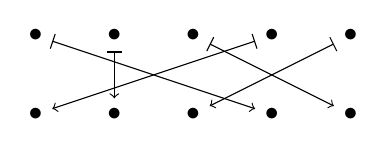
\begin{tikzpicture}
	\useasboundingbox (0.9, -1.1) rectangle (5.1, 0.1);
		\foreach \i in {1,2}{
			\foreach \j in {1,...,5}{
				\node at (\j,1-\i) (N\i\j) {$\bullet$};
			}
		}
		\draw[|->] (N11) -- (N24);
		\draw[|->] (N12) -- (N22);
		\draw[|->] (N13) -- (N25);
		\draw[|->] (N14) -- (N21);
		\draw[|->] (N15) -- (N23);
	\end{tikzpicture}
	\]
It's a do-si-do, a ``partner move,'' where everyone picks a partner (possibly themselves) and exchanges with them. One example one could take $D$ to be the set of pixels in a photograph, and take $s$ to be the function sending each pixel to its mirror image across the vertical center line of the photograph.
  \item We could make $D(c)$ the set of people at a ``secret Santa'' Christmas party, where everyone gives a gift to someone, possibly themselves. Take $D(b)$ to be the set of gifts, $g$ the giver function (each gift is given by a person), and $h$ the receiver function (each gift is received by a person), $D(a)$ is the set of people who give a gift to themselves, and $d(f)\colon D(a)\to D(b)$ is the inclusion.
\end{enumerate}
}

\sol{exc.exponential_cat}{
Let's look more deeply at how $\cat{D}^{\cat{C}}$ is a category.
\begin{enumerate}
	\item Figure out how to compose natural transformations. (Hint: an expert tells you ``for each object $c\in\cat{C}$, compose the $c$-components.'')
	\item Propose an identity natural transformation on any object $F\in\cat{D}^\cat{C}$, and check that it is unital.
\end{enumerate}
}{
\begin{enumerate}
	\item The expert packs so much information in so little space! Suppose given three objects $F,G,H\in\cat{D}^{\cat{C}}$; these are functors $F,G,H\colon\cat{C}\to\cat{D}$. Morphisms $\alpha\colon F\to G$ and $\beta\colon G\to H$ are natural transformations. Most beginners seem to think about a natural transformation in terms of its naturality squares, but the main thing to keep in mind is its components; the naturality squares constitute a check that comes later.\\
	
	So for each $c\in\cat{C}$, $\alpha$ has a component $\alpha_c\colon F(c)\to G(c)$ and $\beta$ has a component $\beta_c\colon G(c)\to H(c)$ in $\cat{D}$. The expert has told us to define $(\alpha\cp\beta)_c\coloneqq(\alpha_c\cp\beta_c)$, and indeed that is a morphism $F(c)\to H(c)$.
	
	Now we do the check. For any $f\colon c\to c'$ in $\cat{C}$, the inner squares of the following diagram commute because $\alpha$ and $\beta$ are natural; hence the outer rectangle does too:
	\[
	\begin{tikzcd}[ampersand replacement=\&]
		F(c)\ar[r, "\alpha_c"]\ar[d, "F(f)"']\&
		G(c)\ar[r, "\beta_c"]\ar[d, "G(f)"']\&
		H(c)\ar[d, "H(f)"']\\
		F(c')\ar[r, "\alpha_c"']\&
		G(c')\ar[r, "\beta_c"']\&
		H(c')
	\end{tikzcd}
	\]
	\item We propose that the identity natural transformation $\id_F$ on a functor $F\colon\cat{C}\to\cat{D}$ has as its $c$-component the morphism $(\id_F)_c\coloneqq \id_{F(c)}$ in $\cat{D}$, for any $c$. The naturality square
		\[
	\begin{tikzcd}[ampersand replacement=\&]
		F(c)\ar[r, "\id_{F(c)}"]\ar[d, "F(f)"']\&
		F(c)\ar[d, "F(f)"]\\
		F(c')\ar[r, "\id_{F(c')}"']\&
		F(c')
	\end{tikzcd}
	\]
obviously commutes for any $f\colon c\to c'$. And it is unital: post-composing $\id_F$ with any $\beta\colon F\to G$ (and similarly for precomposing with any $\alpha\colon E\to F$) results in a natural transformation $\id_F\cp\beta$ with components $(\id_F)_c\cp\beta_c=(\id_{F(c)}\cp\beta_c)=\beta_c$, and this is just $\beta$ as desired.
\end{enumerate}
}

\sol{exc.true_false_preorder_nt}{
Let $\cat{C}$ be an arbitrary category and let $\cat{P}$ be a preorder, thought of as a category. Consider the following statements:
\begin{enumerate}
	\item For any two functors $F,G\colon\cat{C}\to\cat{P}$, there is at most one natural transformation $F\to G$.
	\item For any two functors $F,G\colon\cat{P}\to\cat{C}$, there is at most one natural transformation $F\to G$.
\end{enumerate}
For each, if it is true, say why; if it is false, give a counterexample.
}{
We have a category $\cat{C}$ and a preorder $\cat{P}$, considered as a category.
\begin{enumerate}
	\item Suppose that $F,G\colon\cat{C}\to\cat{P}$ are functors and $\alpha,\beta\colon F\to G$ are natural transformations; we need to show that $\alpha=\beta$. It suffices to check that $\alpha_c=\beta_c$ for each object $c\in\Ob(\cat{C})$. But $\alpha_c$ and $\beta_c$ are morphisms $F(c)\to G(c)$ in $\cat{P}$, which is a preorder, and the definition of a preorder---considered as a category---is that it has at most one morphism between any two objects. Thus $\alpha_c=\beta_c$, as desired.
	\item This is false. Let $\cat{P}\coloneqq\Cat{1}$, let $\cat{C}\coloneqq\fbox{$\LMO{a}\Tto[15pt]{f_1}{f_2}\LMO{b}$}$, let $F(1)\coloneqq a$, let $G(1)\coloneqq b$, let $\alpha_1\coloneqq f_1$, and let $\beta_1\coloneqq g_2$. 
\end{enumerate}
}

\sol{exc.graph_instance}{
In \cref{eqn.free_schema}, a graph is shown (forget the distinction between white and black nodes). Write down the corresponding $\Cat{Gr}$-instance, as in \cref{eqn.sample_Gr_instance}. (Do not be concerned that you are in the primordial ooze.)
}{
We need to write down the following
\[\boxCD{
\begin{tikzcd}[row sep=large, ampersand replacement=\&]
  	\LTO{Employee}\ar[rr, shift left, "\text{WorksIn}"]\ar[dr, bend right, "\text{FName}"']\ar[loop left, "\text{Mngr}"]\&\&
  	\LTO{Department}\ar[ll, shift left, "\text{Secr}"]\ar[dl, bend left, "\text{DName}"]\\
  	\&\LTO[\circ]{string}
\end{tikzcd}
}
\]
as a $\Cat{Gr}$-instance, as in \cref{eqn.sample_Gr_instance}. The answer is as follows:
\[
\begin{tabular}{ r | l l}
  \textbf{Arrow}&\textbf{source}&\textbf{target}\\\hline
	Mngr&Employee&Employee\\
	WorksIn&Employee&Department\\
	Secr&Department&Employee\\
	FName&Employee&string\\
	DName&Department&string\\
\end{tabular}
\hspace{1in}
\begin{tabular}{ r |}
	\textbf{Vertex}\\\hline
	Department\\
	Employee\\
	string\\
	~\\
	~
\end{tabular}
\]
}

\sol{exc.unique_alpha}{
We claim that---with $G,H$ as in \cref{ex.two_graphs_as_instances}---there is exactly one graph homomorphism $\alpha\colon G\to H$ such that $\alpha_{\Set{Arrow}}(a)=d$.
\begin{enumerate}
	\item What is the other value of $\alpha_{\Set{Arrow}}$, and what are the three values of $\alpha_{\Set{Vertex}}$?
	\item In your own copy of the tables of \cref{ex.two_graphs_as_instances}, draw $\alpha_{\Set{Arrow}}$ as two lines connecting the cells in the ID column of $G(\Set{Arrow})$ to those in the ID column of $H(\Set{Arrow})$. Similarly, draw $\alpha_{\Set{Vertex}}$ as connecting lines.
	\item Check the source column and target column and make sure that the matches are natural, i.e.\ that ``alpha-then-source equals source-then-alpha'' and similarly for ``target.''
\end{enumerate}
}{
Let $G,H$ be the following graphs:
\[
G\coloneqq\boxCD{
\begin{tikzcd}[ampersand replacement=\&]
	\LMO{1}\ar[r, "a"]\& \LMO{2}\ar[r, "b"]\& \LMO{3}
\end{tikzcd}
}
\hspace{.7in}
H\coloneqq\boxCD{
\begin{tikzcd}[ampersand replacement=\&]
	\LMO{4}\ar[r, shift right, "c"']\ar[r, shift left, "d"]\& \LMO{5}\ar[loop right, "e"]
\end{tikzcd}
}
\]
and let's believe the authors that there is a unique graph homomorphism $\alpha\colon G\to H$ for which $\alpha_{\Set{Arrow}}(a)=d$.
\begin{enumerate}
	\item We have $\alpha_{\Set{Arrow}}(b)=e$ and $\alpha_{\Set{Vertex}}(1)=4$, $\alpha_{\Set{Vertex}}(2)=5$, and $\alpha_{\Set{Vertex}}(3)=5$.
	\item We roughly copy the tables and then draw the lines (shown in black; ignore the dashed lines for now):
	\[
	\begin{tikzcd}[ampersand replacement=\&, column sep=small, row sep=2pt]
			\&	\&a\ar[ddddll, bend right=10pt]\ar[rr, bend left=20pt, blue, dashed, pos=.6, "t"]	\&1	\&2\ar[drrr, dashed, equal, blue]	\&	\&	\&1\ar[dddll, bend right=10pt]\\
			\&	\&b\ar[ddddll, bend right=10pt]	\&2	\&3	\&	\&	\&2\ar[dddll, bend right=10pt]\\
			\&	\&	\&	\&	\&	\&	\&3\ar[ddll, bend right=10pt]\\
		c	\&4	\&5	\&	\&	\&4	\&	\&\\
		d\ar[rr, bend left=20pt, blue, dashed, pos=.6, "t"]	\&4	\&5\ar[rrr, dashed, equal, blue]	\&	\&	\&5	\&	\&\\
		e	\&5	\&5	\&	\&	\&	\&	\&		
	\end{tikzcd}
	\]
	\item It works! One example of the naturality is shown with the help of dashed blue lines above. See how both paths starting at $a$ end at $5$?
\end{enumerate}
}

\sol{exc.dds_graph}{
Consider the functor $G\colon\Cat{Gr}\to\Cat{DDS}$ given by sending `source' to `next' and sending `target' to the identity on `State'. Migrate the same data, \cref{eqn.state_table}, using $G$. Write down the tables and draw the corresponding graph.
}{
We just need to write out the composite of the following functors
\[
\begin{tikzpicture}[color=blue]
	\node (Arrow) {$\LTO{Arrow}$};
	\node[below=of Arrow] (Vertex) {$\LTO{Vertex}$};
	\draw[->, color=red] 
		($(Arrow.south)+(-3pt,0)$) to node[left, font=\scriptsize] (source) {source} 
		($(Vertex.north)+(-3pt,0)$);
	\draw[->]
		($(Arrow.south)+(3pt,0)$) to node[right, font=\scriptsize] (target) {target} 
		($(Vertex.north)+(3pt,0)$);
	\node[draw, color=black, fit=(Arrow) (Vertex) (source) (target)] (Gr) {};
	\node[below=0 of Gr, black] {$\Cat{Gr}$};
%
	\node[right=2 of target] (State) {$\LTO{State}$} edge [loop below, red] node[font=\scriptsize] (next) {next} ();
	\begin{scope}[color=black]
  	\node[draw, fit=(State) (next)] (DDS) {};
  	\node[below=0 of DDS] {$\Cat{DDS}$};
  %
  	\draw[functor] (Gr.east|-Vertex) to node[above, font=\scriptsize] {$G$} (DDS.west|-Vertex);
  	\node[right=6 of Vertex] (Set) {$\smset$};
  	\draw[functor] (DDS.east|-Vertex) to 
				node[above, font=\tiny] {
 					\begin{tabular}{c | c}
          	\textbf{State}&\textbf{next}\\\hline
          	1 & 4\\
          	2 & 4\\
          	3 & 5\\
          	4 & 5\\
          	5 & 5\\
          	6 & 7\\
          	7 & 6
        \end{tabular}
        }
				(Set.west|-Vertex);
	\end{scope}
\end{tikzpicture}
\]
in the form of a database, and then draw the graph. The results are given below.
\[\footnotesize
	\begin{array}{c | c c}
		\textbf{Arrow}&\textbf{source}&\textbf{target}\\\hline
		1&4&1\\
		2&4&2\\
		3&5&3\\
		4&5&4\\
		5&5&5\\
		6&7&6\\
		7&6&7
	\end{array}
\hspace{.4in}
	\begin{array}{c |}
		\textbf{Vertex}\\\hline
		1\\
		2\\
		3\\
		4\\
		5\\
		6\\
		7
	\end{array}
\hspace{.6in}
	\boxCD{
  \begin{tikzcd}[column sep=15pt, row sep=5, pos=.9, ampersand replacement=\&]
  	\&\LMO{1}\ar[from=dr, "1"]\&\&\LMO{2}\ar[from=dl,"2"']\\
  	\LMO{3}\ar[from=dr, "3"]\&\&\LMO{4}\ar[from=dl, "4"']\&\&\LMO{6}\ar[from=r, bend left, pos=.5, "6"]\&[20pt]\LMO{7}\ar[from=l, bend left, pos=.5, "7"]\\
  	\&\LMO[under]{5}\ar[loop below, looseness=5, pos=.5, "5"]
  \end{tikzcd}
}
\]
}

\sol{exc.currying_practice}{
In \cref{ex.currying}, we discussed an adjunction between functors $-\times B$
and $(-)^B$. But we only said how these functors worked on objects: for any set
$X$, they return sets $X\times B$ and $X^B$ respectively.
\begin{enumerate}
	\item Given a morphism $f\colon X\to Y$, what morphism should $-\times B\colon X\times B\to Y\times B$ return?
	\item Given a morphism $f\colon X\to Y$, what morphism should $(-)^B\colon X^B\to Y^B$ return?
	\item Consider the function $+\colon\NN\times\NN\to\NN$, which sends
	$(a,b)\mapsto a+b$. Currying $+$, we get a certain function
	$p\colon\NN\to\NN^\NN$. What is $p(3)$?
\end{enumerate}
}{
We are interested in how the functors $-\times B$
and $(-)^B$ should act on morphisms for a given set $B$. We didn't specify this in the text---we only specified $-\times B$ and $(-)^B$ on objects---so in some sense this exercise is open: you can make up anything you want, under the condition that it is functorial. However, the authors cannot think of any such answers except the one we give below.
\begin{enumerate}
	\item Given an arbitrary function $f\colon X\to Y$, we need a function $X\times B\to Y\times B$. We suggest the function which might be denoted $f\times B$; it sends $(x,b)$ to $(f(x),b)$. This assignment is functorial: applied to $\id_X$ it returns $\id_{X\times B}$ and it preserves composition.
	\item Given a function $f\colon X\to Y$, we need a function $X^B\to Y^B$. The canonical function would be denoted $f^B$; it sends a function $g\colon B\to X$ to the composite $(g\cp f)\colon B\to X\to Y$. This is functorial: applied to $\id_X$ it sends $g$ to $g$, i.e.\ $f^B(\id_X)=\id_{X^B}$, and applied to the composite $(f_1\cp f_2)\colon X\to Y\to Z$, we have
	\[(f_1\cp f_2)^B(g)=g\cp (f_1\cp f_2)=(g\cp f_1)\cp f_2=(f_1^B\cp f_2^B)(g)\]
	for any $g\in X^B$.
	\item If $p\colon\nn\to\nn^\nn$ is the result of currying $+\colon\NN\times\NN\to\NN$, then $p(3)$ is an element of $\nn^\nn$, i.e.\ we have $p(3)\colon\nn\to\nn$; what function is it? It is the function that adds three. That is $p(3)(n)\coloneqq n+3$.
\end{enumerate}
}

\sol{ex.terminal_cat}{
Describe the functor $!\colon \cat{C} \to \Cat{1}$ from \cref{eqn.terminal_functor}. Where does it send each
object? What about each morphism?
}{
The functor $!\colon \cat{C} \to \Cat{1}$ from \cref{eqn.terminal_functor} sends each object $c\in\cat{C}$ to the unique object $1\in\Cat{1}$ and sends each morphism $f\colon c\to d$ in $\cat{C}$ to the unique morphism $\id_1\colon 1\to 1$ in $\Cat{1}$.
}

\sol{exc.draw_graph}{
Note that $\cat{G}$ from \cref{eqn.graph_email} is isomorphic to the schema $\Cat{Gr}$. In \cref{subsec.instances_cat} we saw that instances on $\Cat{Gr}$ are graphs. Draw
the above instance $I$ as a graph.
}{
We want to draw the graph corresponding to the instance $I\colon\cat{G}\to\smset$ shown below:
\[
\begin{tabular}{ c | c c}
  \textbf{Email}&\textbf{sent\_by}&\textbf{received\_by}\\\hline
	Em\_1 & Bob & Grace\\
	Em\_2 & Grace & Pat\\
	Em\_3 & Bob & Emory\\
	Em\_4 & Sue & Doug\\
	Em\_5 & Doug & Sue\\
	Em\_6 & Bob & Bob
\end{tabular}
\hspace{1in}
\begin{tabular}{ c |}
	\textbf{Address}\\\hline
	Bob\\
	Doug\\
	Emory\\
	Grace\\
	Pat\\
	Sue
\end{tabular}
\]
Here it is, with names and emails shortened (e.g.\ B=Bob, 3=Em\_3):
\[
\boxCD{
\begin{tikzcd}[ampersand replacement=\&,row sep=1.5ex]
  E\&
  B\ar[r, "1"]\ar[l, "3"']\ar[loop above, "6"]\&
  G\ar[r, "2"]\&
  P\&
  S\ar[r, bend left, "4"]\&
  D\ar[l, bend left, "5"]
\end{tikzcd}
}
\]
}

\sol{exc.terminal_in_preorder}{
Let $(P,\le)$ be a preorder, let $z\in P$ be an element, and let $\cat{P}$ be the corresponding category (see \cref{subsubsec.pos_free_spectrum}). Show that $z$ is a terminal object in $\cat{P}$ if and
only if it is a \emph{top element} in $P$: that is, if and only if for all $c \in P$ we have $c \le
z$.
}{
An object $z$ is terminal in some category $\cat{C}$ if, for every $c\in\cat{C}$ there exists a unique morphism $c\to z$. When $\cat{C}$ is the category underlying a preorder, there is at most one morphism between any two objects, so the condition simplifies: an object $z$ is terminal iff, for every $c\in\cat{C}$ there exists a morphism $c\to z$. The morphisms in a preorder are written with $\leq$ signs, so $z$ is terminal iff, for every $c\in P$ we have $c\leq z$, and this is the definition of top element.
}

\sol{exc.terminal_cat}{
What is the terminal object in the category $\smcat$? (Hint: recall
\cref{ex.terminal_cat}.)
}{
The terminal object in $\smcat$ is $\Cat{1}$ because by \cref{ex.terminal_cat} there is a unique morphism (functor) $\cat{C}\to\Cat{1}$ for any object (category) $\cat{C}\in\smcat$.
}

\sol{exc.cat_wo_terminal}{
Not every category has a terminal object. Find one that doesn't.
}{
Consider the graph $2V\coloneqq\fbox{$\bullet\;\bullet$}$ with two vertices and no arrows, and let $\cat{C}=\free(2V)$; it has two objects and two morphisms (the identities). This category does not have a terminal object because it does not have any morphisms from one object to the other.
}

\sol{exc.meet_product}{
Let $(P,\le)$ be a preorder, let $x,y \in P$ be elements, and let $\cat{P}$ be the corresponding category. Show that their product $x\times y$ in $\cat{P}$ agrees with their meet $x\wedge y$ in $P$.
}{
A product of $x$ and $y$ in $\cat{P}$ is an object $z\in\cat{P}$ equipped with maps $z\to x$ and $z\to y$ such that for any other object $z'$ and maps $z'\to x$ and $z'\to y$, there is a unique morphism $z'\to z$ making the evident triangles commute. But in a preorder, the maps are denoted $\leq$, they are unique if they exist, and all diagrams commute. Thus the above becomes: a product of $x$ and $y$ in $\cat{P}$ is an object $z$ with $z\leq x$ and $z\leq y$ such that for any other $z'$, if $z'\leq x$ and $z'\leq y$ then $z'\leq z$. This is exactly the definition of meet, $z=x\wedge y$.
}

\sol{exc.product_cats}{
\begin{enumerate}
  \item What are the identity morphisms in a product category $\cat{C}\times\cat{D}$?
  \item Why is composition in a product category associative?
  \item What is the product category $\Cat{1} \times \Cat{2}$?
  \item What is the product category $\cat{P} \times \cat{Q}$ when $P$ and $Q$ are preorders and $\cat{P}$ and $\cat{Q}$ are the corresponding categories?
\end{enumerate}
}{
\begin{enumerate}
  \item The identity morphism on the object $(c,d)$ in the product category $\cat{C}\times\cat{D}$ is $(\id_c,\id_d)$.
  \item Suppose given three composable morphisms in $\cat{C}\times\cat{D}$
  \[(c_1,d_1)\To{(f_1,g_1)}(c_2,d_2)\To{(f_2,g_2)}(c_3,d_3)\To{(f_3,g_3)}(c_4,d_4).\]
  We want to check that $((f_1,g_1)\cp(f_2,g_2))\cp(f_3,g_3)=
  (f_1,g_1)\cp((f_2,g_2)\cp(f_3,g_3))$. But composition in a product category is given component-wise. That means the left-hand side is $((f_1\cp f_2)\cp f_3, (g_1\cp g_2)\cp g_3)$, whereas the right-hand side is $(f_1\cp(f_2\cp f_3),g_1\cp(g_2\cp g_3))$, and these are equal because both $\cat{C}$ and $\cat{D}$ individually have associative composition.
  \item The product category $\Cat{1} \times \Cat{2}$ has two objects $(1,1)$ and $(1,2)$ and one non-identity morphism $(1,1)\to(1,2)$. It is not hard to see that it looks the same as $\Cat{2}$. In fact, for any $\cat{C}$ there is an isomorphism of categories $\Cat{1}\times\cat{C}\cong\cat{C}$.
	\item Let $P$ and $Q$ be preorders, let $X=P\times Q$ be their product preorder as defined in \cref{ex.product_preorder}, and let $\cat{P}$, $\cat{Q}$, and $\cat{X}$ be the corresponding categories. Then $\cat{X}=\cat{P}\times\cat{Q}$.
\end{enumerate}
}

\sol{exc.prod_as_term_cone}{
Check that a product $X \xleftarrow{p_X} X\times Y\xrightarrow{p_Y} Y$ is
exactly the same as a terminal object in $\Cat{Cone}(X,Y)$.
}{
A product of $X$ and $Y$ is an object $Z$ equipped with morphisms $X\From{p_X} Z\To{p_Y} Y$ such that for any other object $Z'$ equipped with morphisms $X\From{p'_X} Z'\To{p'_Y}Y$, there is a unique morphism $f\colon Z'\to Z$ making the triangles commute, $f\cp p_X=p'_X$ and $f\cp p_Y=p'_Y$. But ``an object equipped with morphisms to $X$ and $Y$'' is exactly the definition of an object in $\Cat{Cone}(X,Y)$, and a morphism $f$ making the triangles commute is exactly the definition of a morphism in $\Cat{Cone}(X,Y)$. So the definition above becomes: a product of $X$ and $Y$ is an object $Z\in\Cat{Cone}(X,Y)$ such that for any other object $Z'$ there is a unique morphism $Z'\to Z$ in $\Cat{Cone}(X,Y)$. This is exactly the definition of $Z$ being terminal in $\Cat{Cone}(X,Y)$.
}

\sol{exc.limit_formula_products}{
Show that the limit formula in \cref{thm.set_limits} works for products. See \cref{ex.prods_as_lims}.
}{
Suppose $\cat{J}$ is the graph $\fbox{$\LMO{v_1}\;\LMO{v_2}$}$ and $D\colon\cat{J}\to\smset$ is given by two sets, $D(v_1)=A$ and $D(v_2)=B$ for sets $A,B$. The product of these two sets is $A\times B$. Let's check that the limit formula in \cref{thm.set_limits} gives the same answer. It says
\begin{multline*}
  \lim_\cat{J} D \coloneqq \big\{(d_1,\ldots,d_n)\mid d_i\in D(v_i)\text{ for all }1\leq i\leq n\text{ and }\\
  \text{for all }a\colon v_i\to v_j\in A, \text{ we have } D(a)(d_i)=d_j\big\}.
\end{multline*}
But in our case $n=2$, there are no arrows in the graph, and $D(v_1)=A$ and $D(v_2)=B$. So the formula reduces to
\[\lim_\cat{J} D \coloneqq \big\{(d_1,d_2)\mid d_1\in A\text{ and }d_2\in B\big\}.
\]
which is exactly the definition of $A\times B$.
}

\sol{exc.opposite_functor}{
Recall from \cref{def.opposite_cat} that every category $\cat{C}$ has an
opposite $\cat{C}\op$. Let $F\colon \cat{C} \to \cat{D}$ be a functor. How
should we define its opposite, $F\op\colon \cat{C}\op \to \cat{D}\op$? That is,
how should $F\op$ act on objects, and how should it act on morphisms?
}{
Given a functor $F\colon \cat{C} \to \cat{D}$, we define its opposite $F\op\colon \cat{C}\op \to \cat{D}\op$ as follows. For each object $c\in\Ob(\cat{C}\op)=\Ob(\cat{C})$, put $F\op(c)\coloneqq F(c)$. For each morphism $f\colon c_1\to c_2$ in $\cat{C}\op$, we have a corresponding morphism $f'\colon c_2\to c_1$ in $\cat{C}$ and thus a morphism $F(f')\colon F(c_2)\to F(c_1)$ in $\cat{D}$, and thus a morphism $F(f')'\colon F\op(c_1)\to F\op(c_2)$. Hence we can define $F\op(f)\coloneqq F(f')'$. Note that the primes ($-'$) are pretty meaningless, we only put them there to differentiate between things that are very closely related.

It is easy to check that our definition of $F\op$ is functorial: it sends identities to identities and composites to composites.
}
	
\finishSolutionChapter

\end{document}
